\renewcommand{\typeRubriek}{loep}		

%%%%%%%%%%%%%%%%%%%%%%%%%%%%%
% informatie voor de auteur %
%%%%%%%%%%%%%%%%%%%%%%%%%%%%%
% de soorten titels opmaakmogelijkheden die de auteur kan gebruiken:
% section
% section*, betekent dat er geen nummer bij gezet wordt
% subsection
% tussentitel
% citaat
% opsomming
% nummering
% bronnen
% kader
% stellingkader (genummerd)
% stellingkadertwee (niet genummerd)
% kleurkader
% werktekst



% twee parameters voor nieuwe rubriek: titel en auteur (die mogen ook leeggelaten worden o.a. voor redactioneel)
\startNieuweRubriek{Meetkunde van 2D naar 3D en hoger}{Luc Van den Broeck\\ Els Vanlommel}

\startcontents[mainsections]		      % om opsomming in inhoudstafel enkel tot loep te beperken
\begin{multicols}{2}                      
\inhoudstafelLoep		                  % om inhoudstafel in te voegen

\widowpenalty10000              % zou nog aan de preamble toegevoegd moeten worden om weduwen te vermijden
\clubpenalty10000               % zou nog aan de preamble toegevoegd moeten worden om wezen te vermijden

%%%%%%%%%%%%%%%%%%%%%%%%%%%%%%%%%%%%%%%%%%%%%%%%%%%%%%%%%%%%%%%%
%%%%%%%%%%%           START VAN DE TEKST               %%%%%%%%%%
%%%%%%%%%%%%%%%%%%%%%%%%%%%%%%%%%%%%%%%%%%%%%%%%%%%%%%%%%%%%%%%%

\section{Inleiding}

Hogere dimensies hebben altijd al tot de verbeelding gesproken. Zowel in de literatuur als in de filmwereld doet men af en toe wilde speculaties over het bestaan van een hogerdimensionaal universum en over ruimtereizen tussen werelden van een andere dimensie. Ook in onze dagelijkse taal gebruiken we de term \emph{dimensie} in verschillende, niet nader gedefinieerde betekenissen: de sociale dimensie van een probleem, de politieke dimensie van een beslissing, een project van een totaal andere dimensie ... In de natuurwetenschappen staat het woord dimensie voor \emph{grootte} of \emph{afmeting} maar ook voor de \emph{eenheid} die gebruikt wordt. Grootheden zonder eenheid, noemen we \emph{dimensieloos}. Over deze betekenissen van het woord \emph{dimensie} gaat het niet in deze loep.

We bekijken dimensies louter wiskundig. Een rechte heeft dimensie 1. Elk punt op deze rechte kan ondubbelzinnig omschreven worden door één coördinaatgetal. Een vlak heeft dimensie twee. Er zijn twee coördinaatgetallen nodig om elk punt vast te leggen. En onze gekende ruimte is driedimensionaal. Tot zover kan iedereen volgen, van jong tot oud. 

Maar als we verder willen gaan wordt het moeilijk zonder strenge wiskundige fundering. Deze fundering kwam er o.a. dank zij de ontwikkeling van de theorie van de vectorruimten. Slechts een heel klein gedeelte van onze huidige leerlingenpopulatie heeft genoeg kennis van vectorruimten om de finesses van de begrippen basis en dimensie te kunnen begrijpen. Af en toe krijgen wij, wiskundeleerkrachten, vragen over het bestaan van een vierde dimensie. En of de vierde dimensie dan de tijd is. En dan verwachten de leerlingen uiteraard een duidelijk antwoord, zonder verwijzingen naar deze abstracte structuren.

Dit brengt ons bij het opzet van deze loep. Het meetkundige begrip \emph{dimensie} kan aan bijna alle leerlingen tot op een zekere hoogte uitgelegd worden zonder het abstractieniveau van een vectorruimte aan te halen. We vermelden in deze loep niet in welk leerjaar je welke benadering kunt aanbrengen. Het is immers ook niet op voorhand duidelijk welke leerlingen belangstelling vertonen voor een uitweiding over dit thema. Het doelpubliek is met andere woorden erg variabel. Om deze reden worden er ook geen werkteksten voorzien in deze loep.   

Zet je dus in je zetel, beste Uitwiskelaar. Lees over 'Meetkunde van 2D naar 3D en hoger'. Markeer wat je boeit en grijp ernaar als je leerlingen interesse vertonen in de hogerdimensionale meetkunde. Je zult zien dat ook de interesse voor de gewone meetkunde bij de modale leerling sterk zal gewekt worden bij een klein uitstapje naar hogere dimensies.

\tussentitel{Wat lees je in deze loep?}

In \emph{paragraaf 2} laten we zien hoe je diepere inzichten krijgt door in de meetkunde een switch te maken naar een hogere dimensie. Deze paragraaf gaat over \emph{Ruimtevisioenen in Platland}, een term die we ontleenden aan Martin Kindt (1993). We behandelen de dimensiesprong van 2D naar 3D. Maar het is evenzeer nuttig af en toe de dimensiesprong van 1D naar 2D te maken. Deze dimensiesprongen op lager niveau zijn een goede voorbereiding voor de dimensiesprong van 3D naar 4D die we verderop zullen maken.

We proberen ons driedimensionale lichamen vaak voor te stellen op basis van een tweedimensionale perspectiefafbeelding. Deze afbeeldingen zijn onvolmaakt. Er gaat heel wat informatie verloren. Hoeken en afmetingen zijn niet altijd wat ze lijken. Snijdingen van rechten kunnen bedrieglijk zijn. Als je weet waarop je kunt vertrouwen, zijn deze symbolische afbeeldingen wel in orde. 
In \emph{paragraaf 3} tonen we enkele technieken om vierdimensionale lichamen af te beelden in een drie- of in een tweedimensionale omgeving. Ook deze afbeeldingen zijn onvolmaakt. Je kunt ze niet gebruiken om er op te meten. Maar ze helpen je bijvoorbeeld wel om het aantal hoekpunten, ribben, zijvlakken en cellen in het vierdimensionale lichaam te tellen.

In de \emph{paragrafen 4 en 5} wordt er gerekend: in de vierde paragraaf met coördinaten, in de vijfde met vectoren. Het uitbreiden van de rekenregels om bijvoorbeeld het midden van een lijnstuk of de afstand tussen twee punten te berekenen, gebeurt op basis van een analogie. Door te rekenen in hogerdimensionale ruimten kunnen we ook stellingen bewijzen als het meetkundige inzicht hiervoor ontbreekt. We hoeven ons de hogerdimensionale ruimte zelfs niet meer te kunnen inbeelden.

\emph{Paragraaf 6} gaat over het boek Flatland dat in 1884 geschreven werd door de Anglicaanse predikant Edwin Abbott Abbott. In dit boek wordt de driedimensionale wereld beschreven door het oog van tweedimensionale wezens en de tweedimensionale door het oog van eendimensionale wezens. Flatland laat zien hoe er vroeger pogingen gedaan werden om inzicht te krijgen in hogere dimensies. Dit is een prima opstapje naar de meetkunde in vier dimensies. Maar, ook al doe je in de klas niet veel met de vierde dimensie, het verhaal van Flatland doet het sowieso bij de leerlingen.

\tussentitel{Wat las je eerder in Uitwiskeling?}

Een tiental jaar geleden schreef Pedro Tytgat (2010) een boeiend spinnenwebartikel naar aanleiding van een klasproject over \emph{Meer dan drie dimensies}. Hierin werden drie methoden voorgesteld om de vierde dimensie te visualiseren: via doorsneden en projecties, via analogieën en via het maken van ontvouwingen. De laatste twee technieken worden in deze loep breed uitgewerkt. Wie Uitwiskeling aandachtig las en een goed geheugen heeft, herkent wellicht enkele dingen.

Ook over de film Flatland (flatlandthemovie) schreef Pedro Tytgat (2009) een korte recentie in Uitwiskeling. In deze verfilming van het boek van Abbott vind je misschien stof voor een samenwerkingsproject met je collega Engels.

\section{Ruimtevisioenen in Platland}

In deze paragraaf bekijken we vlakke problemen vanuit de ruimte. Hierdoor krijgen we soms een bredere kijk op het probleem en vinden we ook soms een snellere oplossing. Martin Kindt (1993) noemde deze werkwijze in een artikel in de Nieuwe Wiskrant een \emph{ruimtevisioen in Platland}. 

Het tegenovergestelde van een \emph{ruimtevisioen in Platland} bestaat ook. Je kunt een driedimensionaal probleem ontleden en oplossen door naar de projectie van dit probleem op een vlak te kijken. Dit illustreren we op het einde van deze paragraaf.

\end{multicols}


\begin{center}
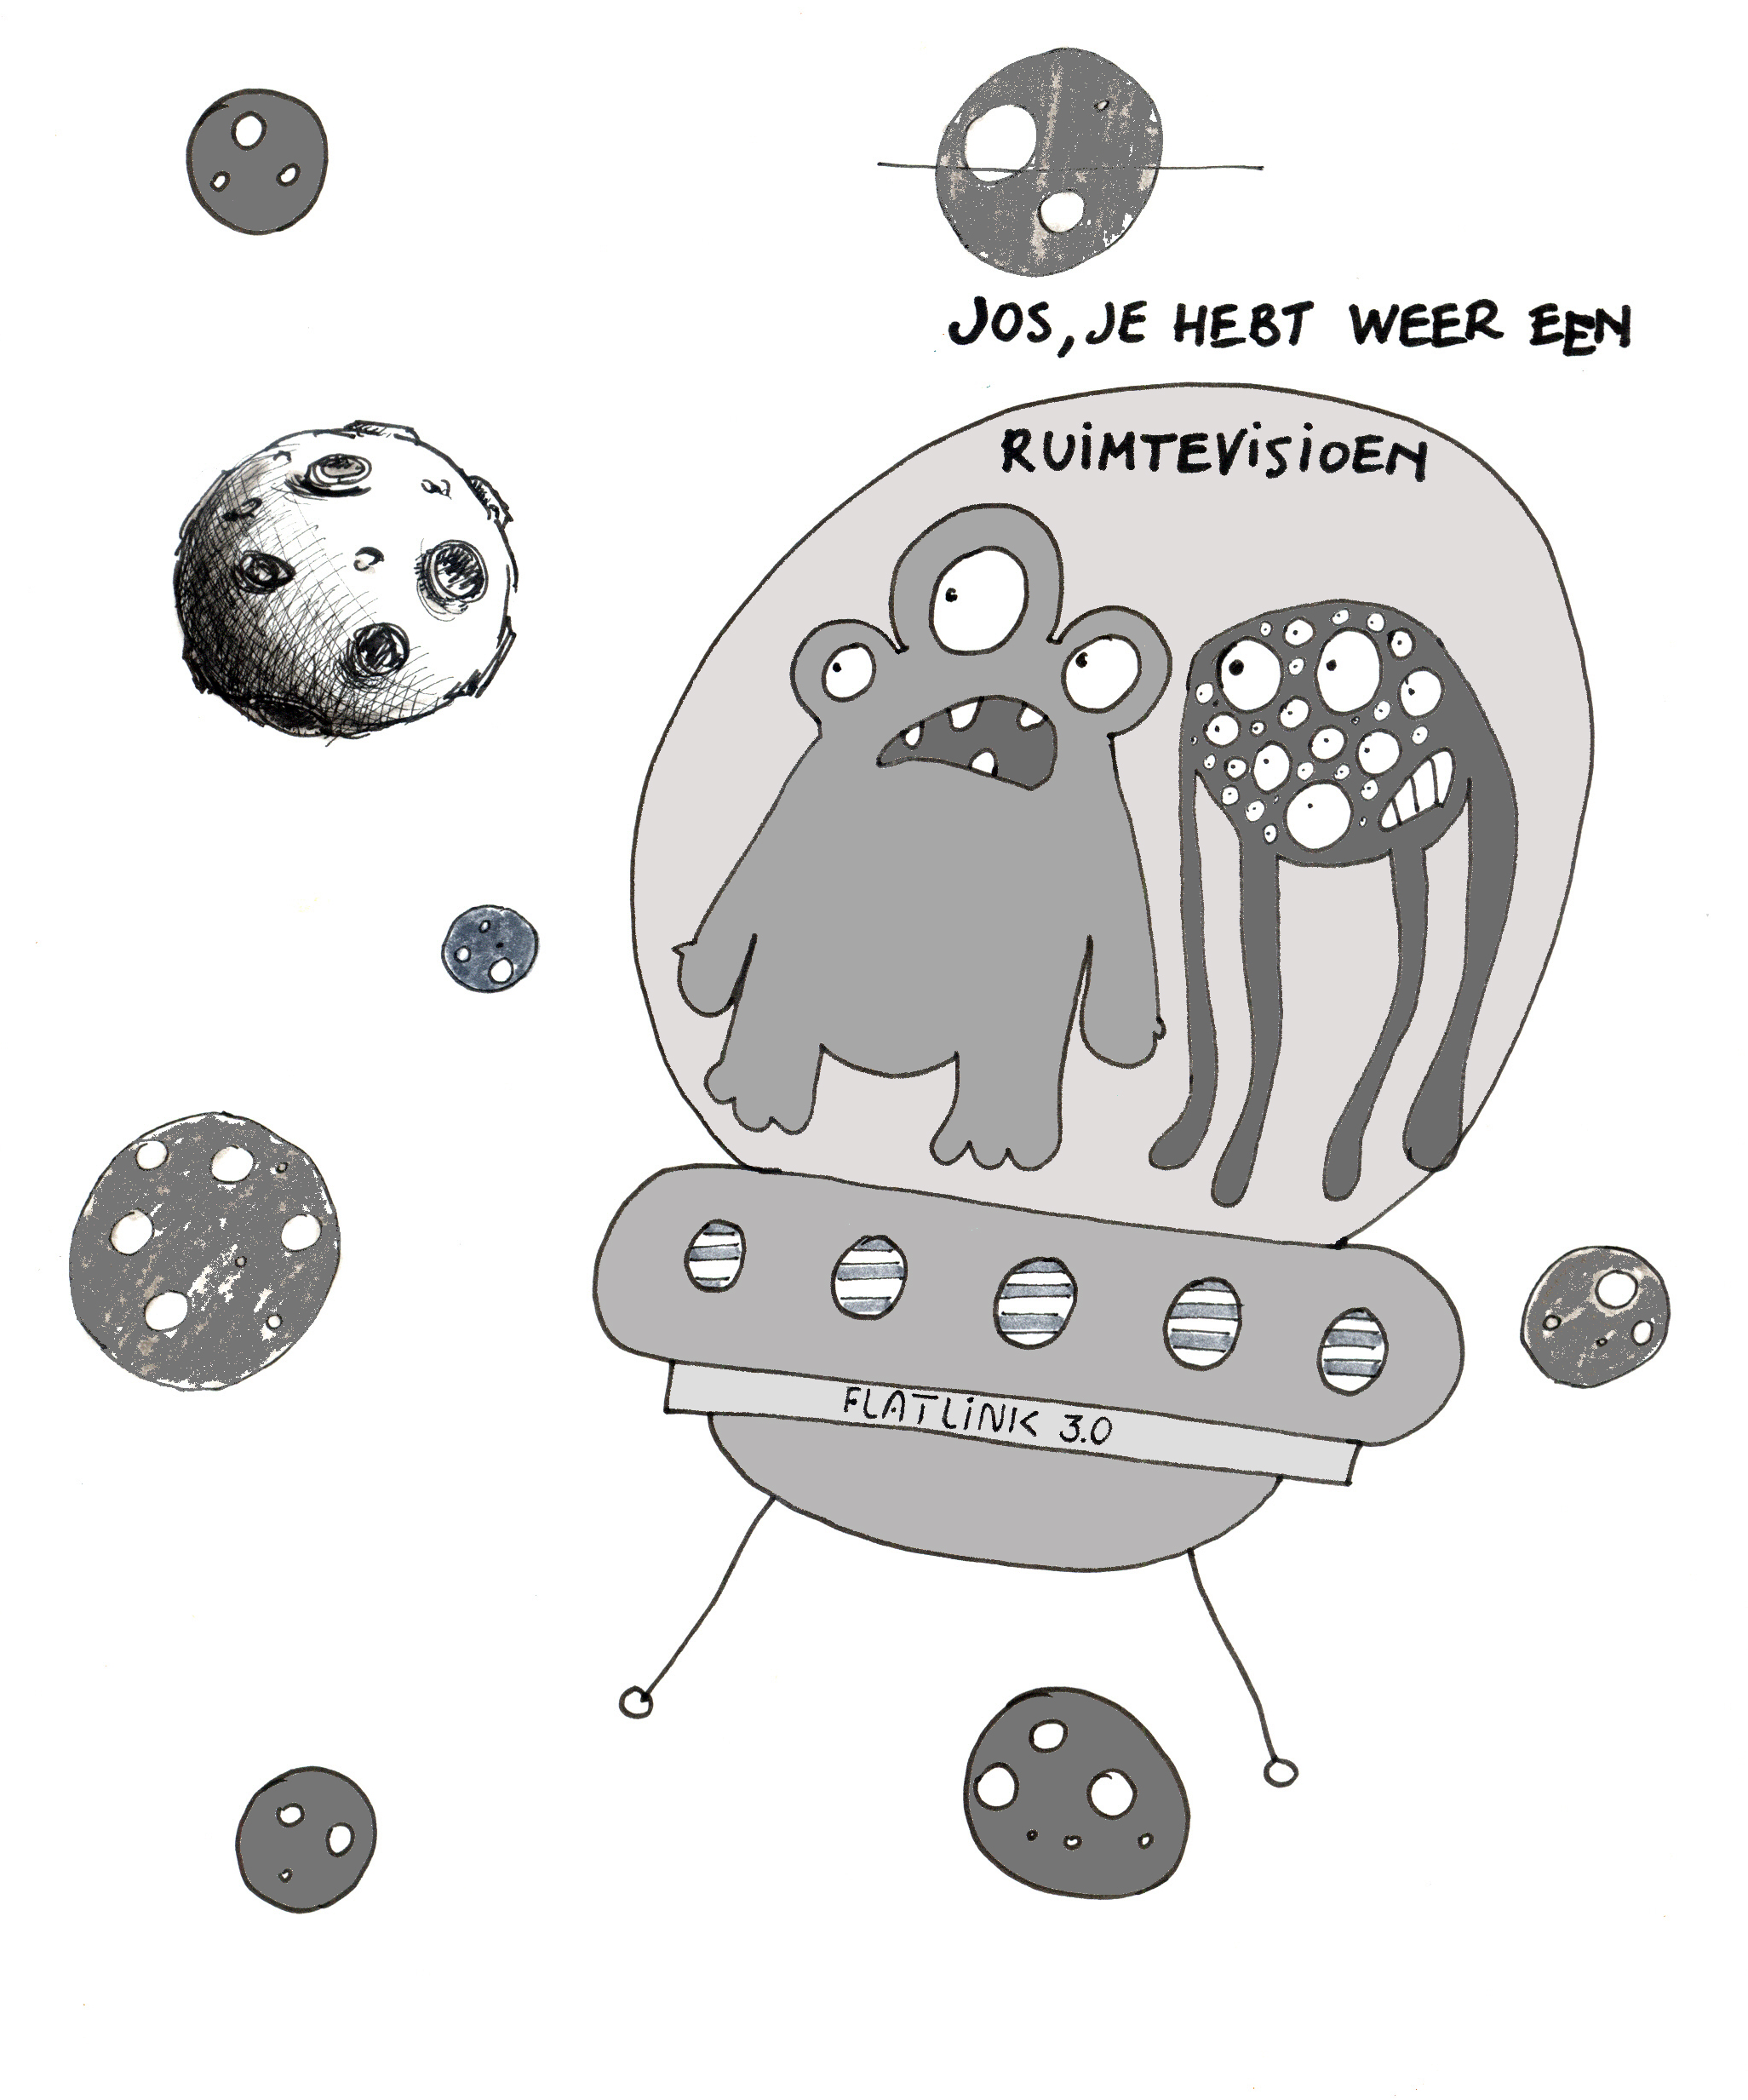
\includegraphics[width=0.8\linewidth]{img/UW mei ruimtevisioen.jpg}
\end{center}

\begin{multicols}{2}

Soortgelijke dimensiesprongen kunnen we maken tussen de driedimensionale en de vierdimensionale ruimte en ook hogerop. Hier gaan we echter niet dieper op in. De bedoeling van deze paragraaf is om de lezer te overtuigen van de zin van dimensiewissels. En hiervoor moeten we beginnen bij de laagste dimensies.

\subsection{De diagonalen van een halfregelmatige zeshoek}

We starten met een zeer eenvoudig probleem. Neem een zeshoek waarvan de overstaande zijden evenwijdig en even lang zijn, zie figuur \ref{fig1}. We zullen een dergelijke zeshoek in deze paragraaf een \emph{halfregelmatige zeshoek} noemen. Toon voor de halfregelmatige zeshoek aan dat de diagonalen elkaar in één punt snijden en dat ze elkaar middendoor snijden. Toon ook aan dat deze zeshoek op twee manieren verknipt kan worden in drie parallellogrammen.

\begin{center}
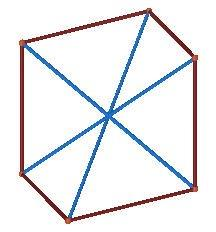
\includegraphics[width=0.5\linewidth]{img/zeshoek1.jpg}
\captionof{figure}{De diagonalen van een halfregelmatige zeshoek}
\label{fig1}
\end{center}

Je kunt deze stelling bewijzen met eenvoudige hulpstellingen uit de vlakke meetkunde. Leg het tijdschrift nu even weg en denk hier onbevangen over na. Het bewijs verloopt directer met een ruimtevisioen. Een halfregelmatige zeshoek, zoals hij hier gedefinieerd werd, is de buitenomtrekslijn van een kubus in evenwijdig perspectief. Dat zie je in figuur \ref{fig2}. De diagonalen van een kubus snijden elkaar middendoor. En verder weten we dat de evenwijdige perspectiefvoorstelling het midden bewaart: het midden van een lijnstuk in de ruimte wordt getekend als het midden van het overeenkomstige perspectieflijnstuk. Klaar.

Ook de tweede bewering is triviaal door de interpretatie vanuit de perspectiefvoorstelling van een kubus. Om van de halfregelmatige zeshoek naar de kubus te gaan, zijn er twee extra punten nodig. Elk van deze punten is een hoekpunt van drie vierkante zijvlakken van de kubus. In de evenwijdige perspectiefvoorstelling hebben deze drie vierkante zijvlakken de vorm van een parallellogram. Opnieuw klaar. 

\begin{center}
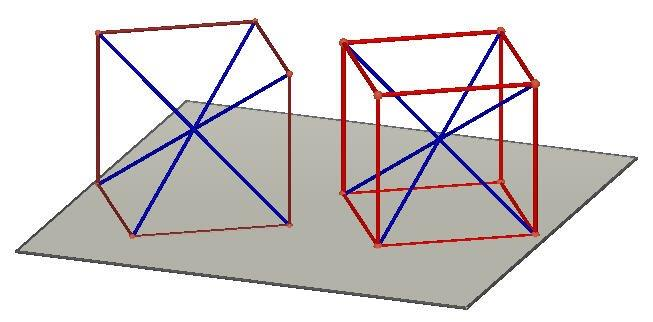
\includegraphics[width=\linewidth]{img/zeshoek.jpg}
\captionof{figure}{Bewijs door een ruimtevisioen}
\label{fig2}
\end{center}

Als je voor het bewijs niet uit het vlak mag of kunt treden, heb je meerdere stappen nodig. Ziehier een voorbeeld van een gewoon bewijs voor de eerste bewering. 

Je kiest eerst twee overstaande zijden die evenwijdig en even lang zijn. Die bakenen een parallellogram af. Je steunt nu op de eigenschap die zegt dat de diagonalen van een parallellogram elkaar middendoor delen. Vervolgens kies je twee andere overstaande zijden die een parallellogram afbakenen. Met hetzelfde argument vinden we weer dat twee diagonalen even lang zijn. Het eerste duo diagonalen is niet helemaal verschillend van het tweede. Er is altijd één gemeenschappelijke diagonaal in de twee duo's. Hieruit volgt dat de drie diagonalen door één punt gaan en dat ze elkaar middendoor delen. 

\begin{center}
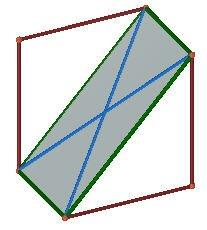
\includegraphics[width=0.5\linewidth]{img/zeshoek2.jpg}
\captionof{figure}{Bewijs zonder het vlak te verlaten}
\label{fig3}
\end{center}

Deze redenering is iets langer. Maar we geven toe, het scheelt niet veel. Hieronder werken we een stelling uit waarbij het verschil tussen de twee bewijsmethoden wel goed merkbaar is.

\subsection{De uitwendige raaklijnen aan drie cirkels}
De Franse wiskundige Gaspard Monge (1746-1818) gaf zijn naam aan een bekende stelling over drie cirkels met hun paren uitwendige raaklijnen, zie figuur \ref{fig4}. We schreven hier eerder al over in Uitwiskeling (zie Roelens, 1992). De stelling gaat als volgt. 

\begin{citaat}
{Drie cirkels met een verschillende straal hebben drie paar uitwendige raaklijnen. De drie snijpunten van de drie paren uitwendige raaklijnen liggen op een rechte.}
\end{citaat}

\begin{center}
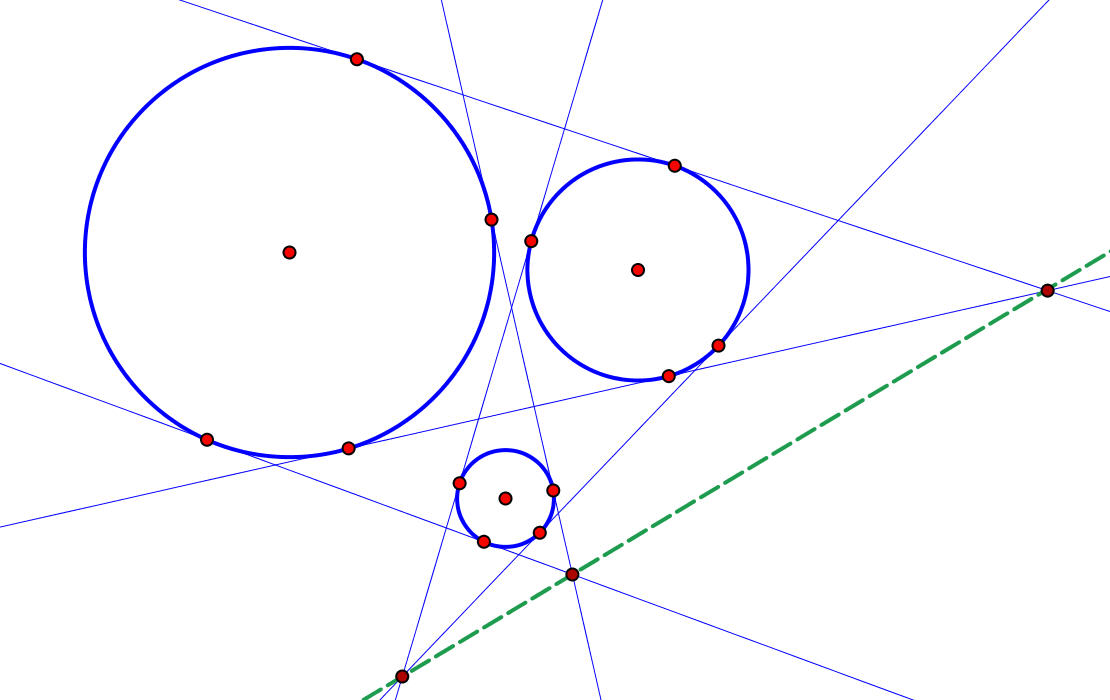
\includegraphics[width=\linewidth]{img/fig4.jpg}
\captionof{figure}{De stelling van Monge}
\label{fig4}
\end{center}

Voor het bewijs met het ruimtevisioen moet je je inbeelden dat de drie cirkels bollen voorstellen die op een bureaublad liggen. Omdat de drie bollen een verschillende straal hebben, kun je elk tweetal bollen verpakken in een kegel, die ook op het bureaublad rust. Beeld je dit in als twee bollen ijs die omklemd worden door een ijshoorntje. 

Het bureaublad is het gemeenschappelijk raakvlak aan de drie kegels. Dit betekent dat de kegels een beschrijvende rechte gemeen hebben met het bureaublad en dat ook hun toppen op het bureaublad liggen. Door deze opstelling is er niet alleen een vlak dat langs onder aan de kegels raakt maar ook een vlak dat langs boven aan de drie kegels raakt. Ook dat vlak bevat de drie toppen. 

Als twee vlakken elkaar snijden in drie punten dan snijden ze elkaar in een hele rechte. De snijrechte van de twee raakvlakken is dus de rechte die de toppen van de kegels bevat. De drie bollen, de drie kegels, het raakvlak langs onder en de snijrechte zie je in figuur \ref{fig5} maar ook, met een beetje verbeelding, in bovenaanzicht in figuur \ref{fig4}, wat het bewijs van de stelling van Monge vervolledigt.

\begin{center}
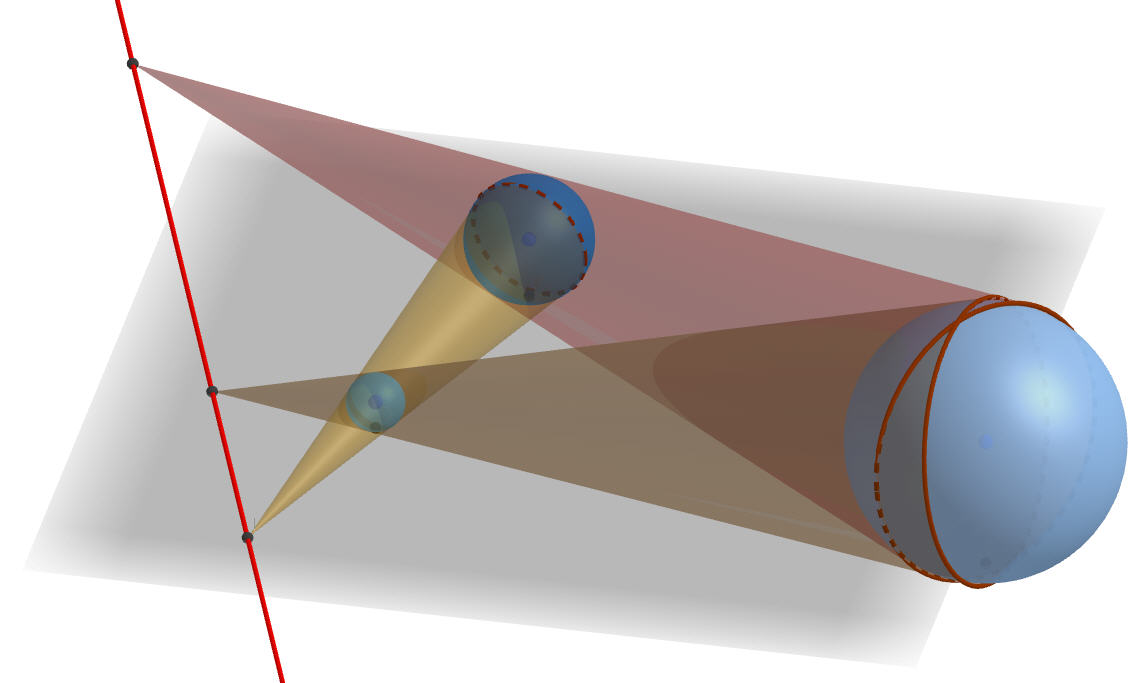
\includegraphics[width=\linewidth]{img/driekegels.jpg}
\captionof{figure}{Bewijs door een ruimtevisioen}
\label{fig5}
\end{center}

Voor het contrast geven we nu een direct bewijs, ontleend aan Gheysens (2012). Noem de middelpunten van de cirkels $P$, $Q$ en $R$ zoals op figuur \ref{fig6}. De stralen zijn achtereenvolgens $r_1$, $r_2$ en $r_3$. De snijpunten van de uitwendige raaklijnen noemen we $A$, $B$ en $C$.

We starten het bewijs met een constructie. Klem een kopie van de kleinste cirkel tussen de uitwendige raaklijnen van de grootste twee cirkels. Noem het middelpunt $S$. De straal van deze cirkel is $r_3$. We tonen nu aan dat het lijnstuk $[RS]$ evenwijdig is met de rechte $BC$ en met de rechte $AC$. Hieruit volgt dan dat $A$, $B$ en $C$ collineair zijn.

Door de gepaste gelijkvormige driehoeken te zoeken (spoor ze op en bewijs dat ze gelijkvormig zijn!) vinden we dat:
\[ \frac{\abs{BP}}{\abs{BR}} = \frac{r_1}{r_3}\]
en dat:
\[ \frac{\abs{CP}}{\abs{CS}} = \frac{r_1}{r_3}.\]
Hieruit volgt de evenredigheid
\[ \frac{\abs{BP}}{\abs{BR}} = \frac{\abs{CP}}{\abs{CS}} \]
die nodig is om de omgekeerde stelling van Thales toe te passen in
driehoek $BCP$. Het besluit van deze stelling is dat $RS \parallel BC$. Op analoge manier kunnen we aantonen dat $RS \parallel AC$. We passen hiervoor de omgekeerde stelling van Thales toe in driehoek $ACQ$.

\begin{center}
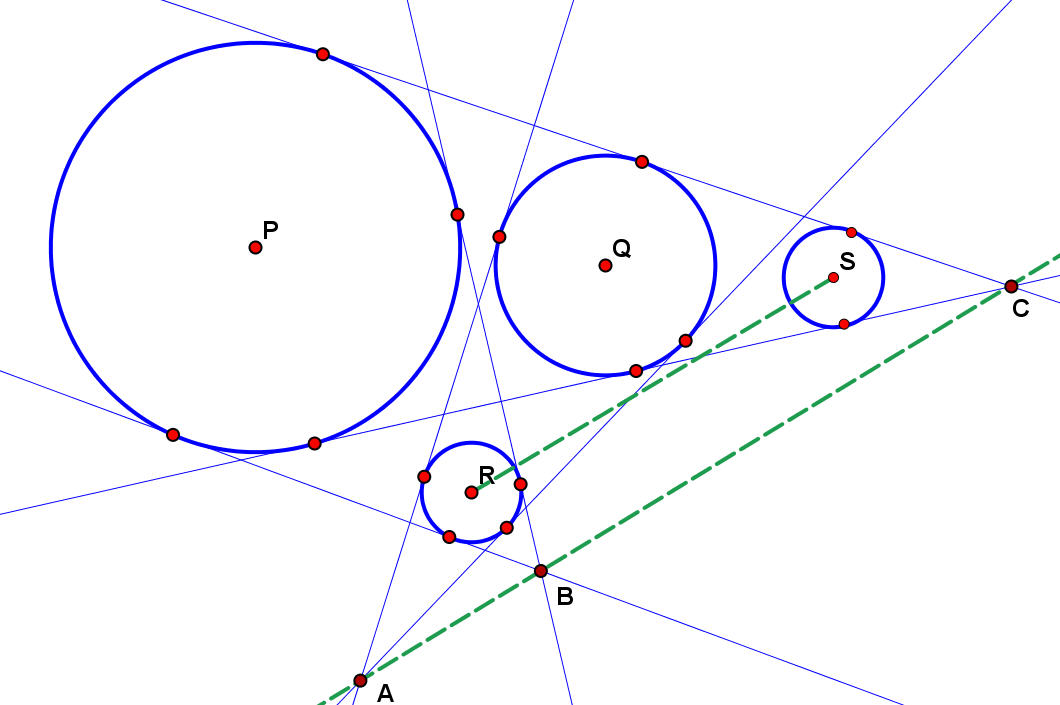
\includegraphics[width=\linewidth]{img/fig6.jpg}
\captionof{figure}{Bewijs zonder het vlak te verlaten}
\label{fig6}
\end{center}

Er zijn nog heel wat andere bewijzen van de stelling van Monge bekend. Ze steunen op minder gekende wiskundige stellingen zoals de stelling van Desargues en de stelling van Menelaos. Liefhebbers van transformaties bewijzen de stelling met: de samengestelde van twee homothetieën met verschillende centra en factoren die niet elkaars omgekeerde zijn, is een nieuwe homothetie waarvan het centrum op één rechte ligt met de twee gegeven centra. 

Voor het ruimtevisioen in Platland is al deze voorkennis niet nodig. Dit is de charme van een bewijs vanuit een hogere dimensie. 

\subsection{Het omgekeerde van een ruimtevisioen in Platland}

Stellingen over tweedimensionale configuraties kun je bewijzen door je kennis te gebruiken van de driedimensionale ruimte. Dat hebben we net geïllustreerd. Maar het kan ook andersom. Als je genoeg vlakke observaties doet, kun je hieruit driedimensionale conclusies trekken. 

In deze paragraaf geven we een voorbeeld van deze werkwijze. We vergeten even waaraan de oppervlakte van een kubus gelijk is. Meer nog, we vergeten dat we in een driedimensionale ruimte leven en we kijken vervolgens als platlanders naar de loodrechte projectie op een vlak van een rondtollende kubus. Hieruit leiden we een formule voor de oppervlakte van de kubus af. Dit klinkt je vreemd in de oren? Lees dan zeker even verder.

Stel dat je een houten kubus hebt met ribbe 1 die je laat rondtollen boven een vast vlak en dat je zijn loodrechte projectie op dit vlak observeert. Je kunt je deze projectie inbeelden als een schaduw met de zon in het zenit. De loodrechte projectie van deze kubus zal variëren van een regelmatige zeshoek naar een halfregelmatige zeshoek (zie figuur \ref{fig7}), naar een rechthoek (zie figuur \ref{fig8}) en in een extreme stand tot een vierkant.

\begin{center}
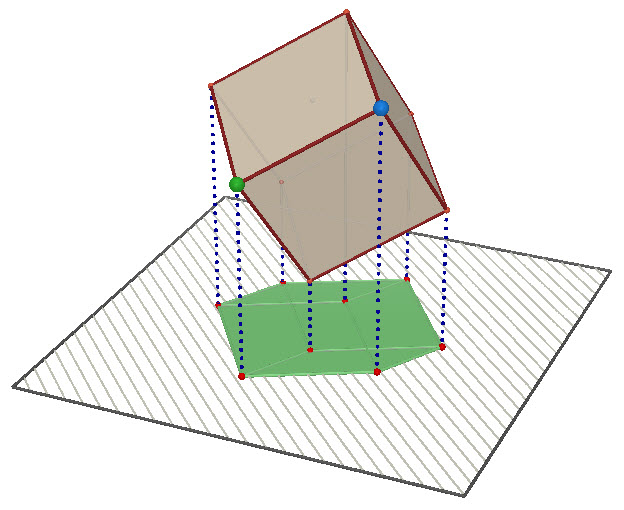
\includegraphics[width=\linewidth]{img/fig7.jpg}
\captionof{figure}{De schaduw is een halfregelmatige zeshoek}
\label{fig7}
\end{center}

\begin{center}
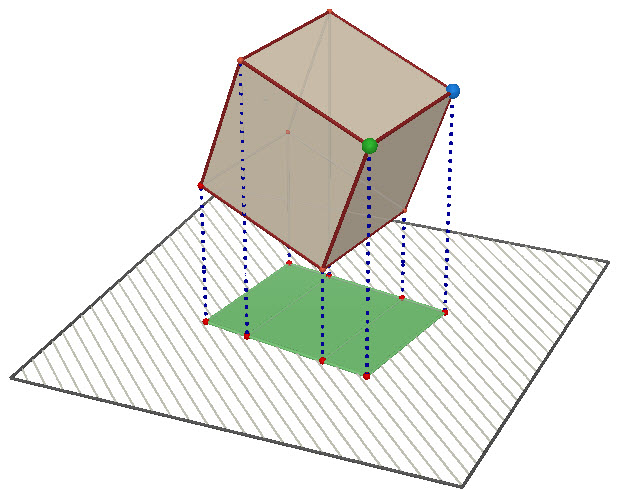
\includegraphics[width=\linewidth]{img/fig8.jpg}
\captionof{figure}{De schaduw is een rechthoek}
\label{fig8}
\end{center}

Als je de projectieoppervlakte opmeet, dan merk je dat die varieert tussen 1 (in het geval van een vierkante schaduw) en $\sqrt{3}$ (in het geval van een regelmatige zeshoek als schaduw). De gemiddelde oppervlakte van de projectie kan niet berekend worden door alleen rekening te houden met deze uiterste waarden, 1 en $\sqrt{3}$. Voor de berekening van de gemiddelde projectieoppervlakte moet je rekening houden met alle mogelijke oriëntaties van de kubus.

Mocht een driedimensionaal wezen je als Platlander willen assisteren, dan kan die ervoor zorgen dat alle oriëntaties van de tollende kubus evenveel kans hebben om voor te komen. Hoe hij dat doet, is moeilijk in te beelden. Maar het kan. Dat leggen we zeker nog eens uit in een spinnenwebartikel. 

Veronderstel dat je erin slaagt om, door de schaduw van de kubus in zeer veel momentopnamen op te meten, de gemiddelde schaduwoppervlakte van de kubus berekenen. Je komt dan uit op 1,5. Vreemd genoeg kun je hieruit dan iets besluiten over de oppervlakte van het ruimtelichaam, zelfs al weet je niet eens dat het om een kubus gaat. Je maakt hiervoor gebruik van de volgende stelling van Cauchy:

\begin{citaat}
{De oppervlakte van een convex ruimtelichaam is vier keer zo groot als de gemiddelde oppervlakte van de loodrechte projectie op een vlak.}
\end{citaat}

Hierdoor zou meteen duidelijk moeten zijn dat de schaduw afkomstig is van een lichaam met oppervlakte 6. 

De Franse wiskundige Augustin-Louis Cauchy (1789-1857) bewees deze stelling in publicaties uit 1841 en 1850. Dit bewijs drong niet door in brede wetenschappelijke kringen. Rond het begin van de twintigste eeuw werd de stelling opnieuw bewezen door de Duitse astronoom  Karl Schwarzschild, die zich bezig hield met dubbelsterren en zwarte gaten. Na de tweede wereldoorlog werd de stelling nog een keer bewezen door Karl Schwarzschilds zoon, die niets afwist van de ontdekking van zijn vader. 

Recent zijn er varianten op de stelling van Cauchy gevonden voor projecties vanuit willekeurige hogerdimensionale ruimten (Slepian, 2012).

Een bewijs van deze stelling in Uitwiskeling hou je nog tegoed. In deze loep zou het de rode draad een beetje teveel onderbreken. 

Een controle van de stelling van Cauchy is de oppervlakteberekening van de bol. De loodrechte projectie van een bol op een vlak is een cirkel, congruent met de evenaarscirkel van de bol. Vermits deze projectie onafhankelijk is van de oriëntatie van de bol, zal de gemiddelde projectie ook gelijk zijn aan de oppervlakte van de evenaarscirkel. En via de stelling van Cauchy zou de oppervlakte van de bol gelijk moeten zijn aan vier keer de oppervlakte van de evenaarscirkel. Klopt.

\begin{center}
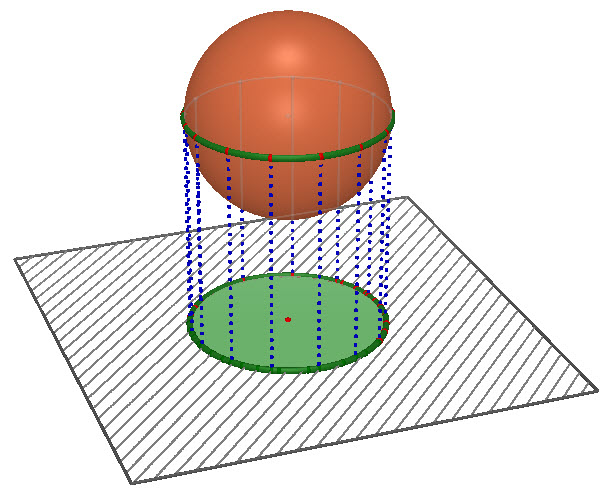
\includegraphics[width=\linewidth]{img/bolencirkel.jpg}
\captionof{figure}{De schaduw van een bol}
\label{fig9}
\end{center}



\section{Voorstellingswijzen van vierdimensionale lichamen}
Sinds onze prille jaren zijn we gewoon ons driedimensionale figuren voor te stellen via een vlakke afbeelding. Deze tekeningen zijn symbolisch. Onze hersens moeten ze immers interpreteren. Ze zijn hier vrij goed in. We weten uit de context dat evenwijdig niet altijd evenwijdig is. En dat hoeken en lengten niet altijd waarheidsgetrouw afgebeeld worden.  Maar er zijn ook zekerheden. Als rechten elkaar in de driedimensionale ruimte snijden, dan snijden ze elkaar ook in de vlakke perspectiefafbeelding. Het omgekeerde is echter niet waar. Snijdende rechten in een vlakke perspectiefafbeeldingen kunnen kruisende rechten in de driedimensionale ruimte voorstellen. Ook van deze schijnbare snijpunten zijn we ons bewust. Dit onderwerp komt ook aan bod in de leerplannen wiskunde van de eerste graad.

Kunnen we leven met deze imperfecte voorstellingen van driedimensionale objecten? Ja hoor, zelfs figuren die getekend zijn met onvolmaakte perspectieftechnieken, kunnen we interpreteren. Denken we bijvoorbeeld aan schilderijen van de Vlaamse Primitieven. Of aan de Egyptische kunst, waarbij we alleen kunnen vertrouwen op een correcte weergave van achter, voor, op en onder. Ook deze afbeeldingen kunnen we vlot interpreteren. 

\begin{center}
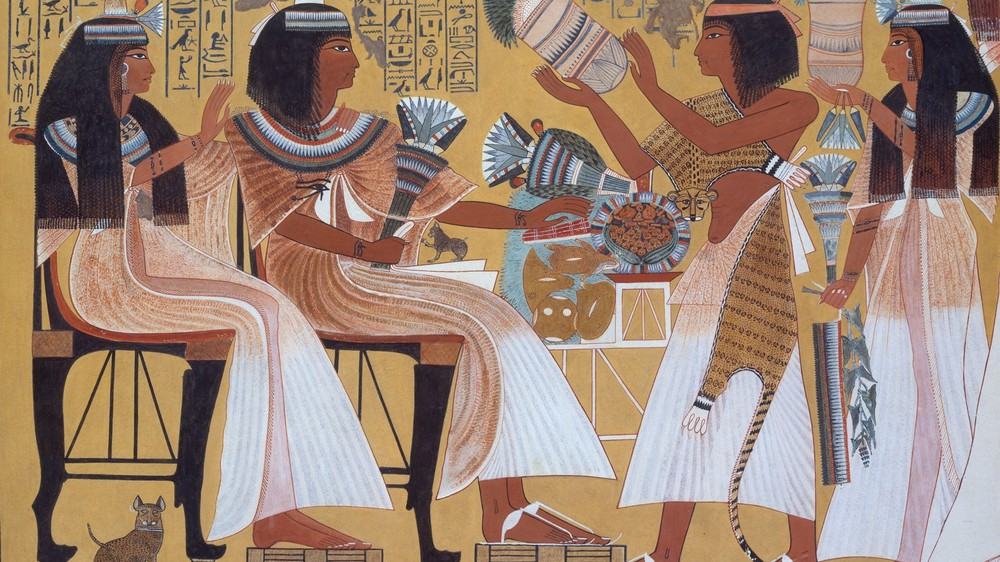
\includegraphics[width=\linewidth]{img/fig10.jpeg}
\captionof{figure}{Ipuy en zijn vrouw krijgen offergaven van hun kinderen (1250 voor Christus)}
\label{fig10}
\end{center}

Verderop in deze paragraaf maken we voorstellingen van vierdimensionale figuren op een tweedimensionale gegevensdrager, bijvoorbeeld op een blad papier. Je mag er hetzelfde van verwachten als bij primitieve en moderne perspectieftekeningen. Eigenschappen van figuren kunnen gewijzigd worden in een vlakke voorstelling. Welke eigenschappen er behouden worden en welke er sneuvelen, kun je pas zeggen als je weet welke techniek je gebruikt om vierdimensionale lichamen voor te stellen.

We belichten twee technieken om vierdimensionale lichamen voor te stellen. De eerste is de voorstelling van een hogerdimensionaal lichaam door een verschuiving van een lagerdimensionaal lichaam. De tweede manier maakt gebruik van lagerdimensionale lichamen die aan elkaar gekleefd en daarna elastisch dichtgevouwen.  

\subsection{Tesseracten voorstellen via verschuivingen}

Een \emph{tesseract} is de wiskundige benaming voor een vierdimensionale kubus. Er zijn verschillende manieren om tesseracten symbolisch voor te stellen in een tweedimensionale tekening. Hieronder laten we de verschuivingsmethode zien.

\tussentitel{ Verschuiven in een hogere dimensie}

We starten met een eenheidslijnstuk. Dat is het eendimensionale equivalent van een kubus. De eindpunten van dit lijnstuk kunnen we coördinaten 0 en 1 geven.

\begin{center}
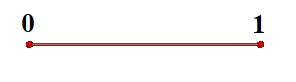
\includegraphics[width=0.5\linewidth]{img/lijnstuk.jpg}
\captionof{figure}{Een eendimensionale kubus}
\label{eenheidslijnstuk}
\end{center}

Door dit lijnstuk in het vlak in de gepaste richting (loodrecht op het lijnstuk) en over een gepaste afstand (die gelijk is aan de lengte van het lijnstuk) te verschuiven, ontstaat er een vierkant. Dit vierkant beschouwen we als een tweedimensionale kubus. De hoekpunten van de tweedimensionale kubus worden aangeduid met twee coördinaatgetallen. Bij de uiteinden van het originele lijnstuk is het tweede coördinaatgetal 0 en bij de uiteinden van het duplicaat 1, zie de grijze coördinaatgetallen in figuur \ref{fig11}.

\begin{center}
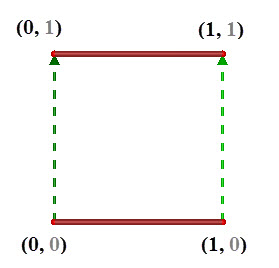
\includegraphics[width=0.6\linewidth]{img/fig11.jpg}
\captionof{figure}{Een tweedimensionale kubus}
\label{fig11}
\end{center}

Vervolgens kunnen we het vierkant verder verschuiven in een gepaste richting (loodrecht op het vierkant) en over een gepaste afstand (die gelijk is aan een zijde van het vierkant). Zo ontstaat een kubus. In figuur \ref{fig12} zie je dat de hoekpunten aangeduid worden met drie coördinaten. Bij de hoekpunten van het originele vierkant is het derde coördinaatgetal 0 en bij de hoekpunten van het duplicaat 1.

\begin{center}
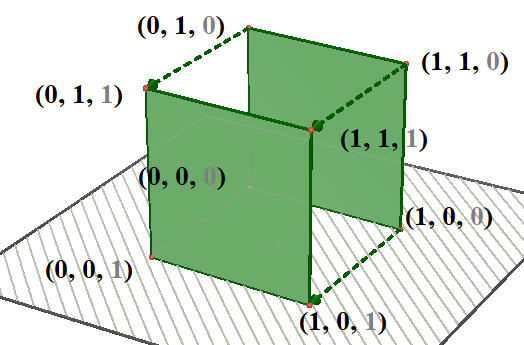
\includegraphics[width=0.9\linewidth]{img/tweedeverschuiving.jpg}
\captionof{figure}{Een driedimensionale kubus}
\label{fig12}
\end{center}

We gaan nog een stapje verder door deze kubus over een gepaste richting (loodrecht op de kubus) en over een gepaste afstand (die gelijk is aan de ribben van de kubus) te verschuiven. Een richting die loodrecht staat op de drie hoofdrichtingen van de kubus, kunnen we ons niet voorstellen in onze dagelijkse omgeving die zich beperkt tot drie dimensies. Vandaar dat we ze voorstellen door een willekeurige verschuiving in onze driedimensionale leefwereld, zie figuur \ref{fig13}. Op welke manier er een vierde coördinaatgetal wordt ingevoerd, wordt ook duidelijk in deze figuur.

\begin{center}
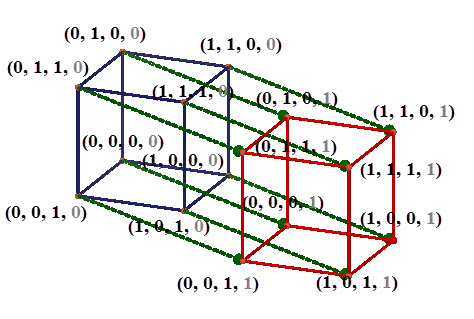
\includegraphics[width=\linewidth]{img/verschuiving2.jpg}
\captionof{figure}{Een vierdimensionale kubus}
\label{fig13}
\end{center}


Deze eenvoudige voorstelling van de vierdimensionale hyperkubus of de tesseract, kun je al uitleggen aan leerlingen van de tweede graad wanneer ze je de vraag stellen hoe we ons de vierde dimensie kunnen voorstellen. Een strakke definitie van het begrip dimensie is op deze leeftijd nog niet mogelijk. Deze benadering is een geschikt alternatief. Zelfs het tekenen van een vijfdimensionale hyperkubus lukt op deze manier als je beschikt over een groot tekenblad en veel geduld. Als je er eentje wilt zien, blader dan even door naar 4.5. Daar hebben we een vijfdimensionale hyperkubus afgebeeld om het begrip Hamming-afstand te illustreren.

Het zal je als lezer niet ontgaan zijn dat we de nuldimensionale objecten nog niet vermeld hebben. Hier is het geschikte ogenblik aangebroken om de allerlaagste dimensie te kijken. Een kubus in een nuldimensionale ruimte is een punt. Op dezelfde manier als hierboven, kun je een nuldimensionale kubus door een verschuiving laten overgaan in een eendimensionale kubus. Het origineel krijgt coördinaat 0 en het duplicaat krijgt coördinaat 1. Zo verklaren we de voorstellingswijze van de nuldimensionale kubus in het systeem. 

\tussentitel{Tellen van deelobjecten}

Als je goed naar figuur \ref{fig13} kijkt, dan kun je makkelijk het aantal hoekpunten, ribben, zijvlakken en kubussen tellen in een hyperkubus. Misschien kun je ze ook structureel tellen, d.w.z. dat je een redenering opbouwt die je kunt verderzetten naar hogere dimensies ... Dat is de bedoeling van dit combinatorisch onderzoek.

Het aantal hoekpunten van de tesseract is 16, precies het dubbele van het aantal hoekpunten van de gewone kubus. Er zijn 8 hoekpunten van de oorspronkelijke kubus en 8 van de verschoven kubus. Het systeem van het verdubbelen van het aantal hoekpunten als je naar een kubus in een hogere dimensie opschuift, is duidelijk. We onthouden dit voor de overgang naar de vijfde dimensie.

Vervolgens tellen we het aantal ribben in de tesseract. Dat zijn er 32. Er waren er 12 in de oorspronkelijke kubus, 12 in de verschoven kubus en dan kwamen er nog 8 bij door de verschuiving van de hoekpunten. De baan van elk hoekpunt tijdens het verschuivingsproces is een lijnstuk. Het systeem achter de telling? Verdubbel het aantal ribben van de driedimensionale kubus en tel er het aantal hoekpunten bij. Zo krijg je het aantal ribben in de vierdimensionale kubus. Ook dit principe onthouden we.

Voor het aantal zijvlakken van de tesseract gaan we vrij analoog te werk. Er zijn 24 zijvlakken in een tesseract. Er waren er 6 in de oorspronkelijke kubus, 6 in de verschoven kubus en 12 zijvlakken ontstonden door het spoor van de 12 ribben van de kubus tijdens de verschuiving. Het systeem? Verdubbel het aantal zijvlakken van de kubus en tel er het aantal ribben bij op. Ook te onthouden.

En nu de moeilijkste: het aantal kubussen in de tesseract. Eerst hebben we de oorspronkelijke kubus en de verschoven kubus. Dat zijn er samen twee. En verder zullen alle zijvlakken een spoor nalaten tijdens de verschuiving. Dat spoor is een kubus. Zo ontstaan er nog 6 extra kubussen. In totaal bevat een tesseract 8 gewone kubussen. Dit getal bepaal je door het dubbel te nemen van het oorspronkelijke aantal kubussen en daar het aantal zijvlakken van de oorspronkelijke kubus bij op te tellen. Dit is een laatste principe dat we verder nodig zullen hebben.

Met gelijkaardige redeneringen kunnen ook de aantallen deelobjecten berekend worden in kubussen in de vijfdimensionale ruimte en hoger. Dat zie je in de tabel (figuur 15). 



Elk getal in de kolom van de hoekpunten is het dubbele van zijn bovenbuur. Alle andere getallen zijn het dubbele van hun bovenbuur vermeerderd met de linkerbovenbuur. Merk op dat de opbouw van deze tabel zeer veel weg heeft van de driehoek van Pascal. Met deze tabel achterhaal je zonder gebruik te maken van combinatorische formules dat bijvoorbeeld een zesdimensionale kubus 192 ribben heeft, en dat een vijfdimensionale kubus 40 gewone kubussen bevat.

Er bestaat ook een combinatorische redenering om het aantal $k$-dimensionale hyperkubussen te tellen in een $n$-dimensionale hyperkubus. Ze is spitsvondig maar ze vraagt ook wat meer inzicht.

Neem een vast hoekpunt van de $k$-dimensionale kubus en identificeer dit hoekpunt met een van de hoekpunten van de $n$-dimensionale kubus. Er zijn $2^n$ mogelijkheden om dit te doen want een $n$-dimensionale kubus heeft $2^n$ hoekpunten. Dat zag je in de eerste kolom van de tabel (figuur 15).

Draai de $k$-dimensionale kubus vervolgens zo om het geïdentificeerde hoekpunt dat zijn ribben samenvallen met ribben van de $n$-dimensionale kubus. Vermits er bij een $k$-dimensionale kubus telkens $k$ ribben in een hoekpunt samenkomen en bij een $n$-dimensionale kubus telkens $n$, is het aantal mogelijkheden gelijk aan het aantal combinaties van $k$ uit $n$:
\[C_n^k=\frac{n!}{k! \cdot (n-k)!}.\]

\end{multicols}

\begin{tabular}{|c|cccccc|}
  \hline
  \begin{tabular}[t]{@{}lr@{}}
           & Elementen: \\
    Dimensie: &
  \end{tabular}  & hoekpunten & ribben & vierkanten & kubussen & 4D-kubussen & 5d-kubussen \\
  \hline
  0  &1   &0  &0   &0     &0     &0  \\
  1  &2   &1  &0   &0     &0     &0  \\
  2  &4   &4  &1   &0     &0     &0  \\
  3  &8   &12  &6   &1     &0     &0  \\
  4  &16   &32  &24   &8     &1     &0  \\
  5  &32   &80  &80   &40    &10    &1  \\
  6  &64   &192 &240  &160   &60    &12  \\
  \hline
\end{tabular}
\captionof{figure}{Overzicht van aantal elementen in een n-dimensionale hyperkubus}

\begin{multicols}{2}
\setlength{\parskip}{1em}

In totaal zijn er $C_n^k \cdot 2^n$ manieren om een $k$-dimensionale kubus met een vast hoekpunt in een $n$-dimensionale kubus in te bedden. 

Bij deze telling wordt elke inbedding meermaals geteld. Je kunt de inbedding van de $k$-dimensionale kubus immers opstarten vanuit elk van de $2^k$ hoekpunten. Daarom moeten we het aantal mogelijkheden nog delen door $2^k$. Het uiteindelijke aantal mogelijkheden is dan gelijk aan
\[C_n^k \cdot 2^{n-k}.\]

Reken maar na. Deze formule geeft eenzelfde uitkomst op de vraag hoeveel lijnstukken (ribben) er in een zesdimensionale hyperkubus zitten:
\[C_6^1 \cdot 2^{6-1}=6\cdot32=192.\]


\subsection{Simplexen voorstellen via aankleven en dichtvouwen}

Een $n$-simplex is het lichaam dat in een $n$-dimensionale ruimte kan geconstrueerd worden door $n+1$ punten (die niet samen in een lagerdimensionale ruimte gelegen zijn) twee aan twee met ribben te verbinden. Een eenvoudiger $n$-dimensionaal object bestaat er niet. Daarom noemen we het simplex een simplex. Simplex is de Latijnse term voor enkelvoudig of eenvoudig.

Een 0-simplex is een punt. Een 1-simplex is een lijnstuk. Een 2-simplex is een driehoek, een 3-simplex een viervlak. Maar hoe gaat het verder? We laten het zien met de methode van aankleven en dichtvouwen. 

\tussentitel{Aankleven en dichtvouwen}

Neem een 1-simplex, in dit voorbeeld het lijnstuk $[AB]$.  Kleef aan de uiteinden van dit lijnstuk en op de rechte $AB$ twee voor de eenvoud even lange lijnstukken, $[AC]$ en $[BD]$. De rechte $AB$ ligt in een vlak. In dit vlak kun je de buitenste lijnstukken scharnierend naar elkaar toe bewegen. Voer deze scharnierbeweging in gedachte uit tot het punt $C$ samenvalt met het punt $D$. Zo ontstaat een 2-simplex, de driehoek $ABC$, zie figuur \ref{dichtplooien1}. 

\begin{center}
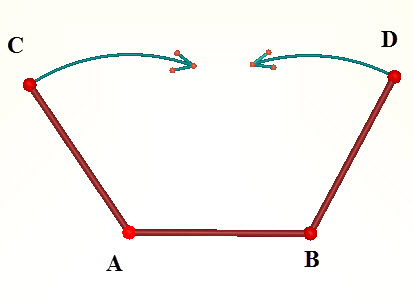
\includegraphics[width=0.8\linewidth]{img/dichtplooien1.jpg}
\captionof{figure}{Simplex: van 1D naar 2D}
\label{dichtplooien1}
\end{center}

Geen enkele leerling zal het moeilijk vinden zich deze scharnierbeweging voor te stellen. Leerlingen leven immers in een hogerdimensionale ruimte en kijken met gemak neer op de tweedimensionale ruimte.


Vanuit een 2-simplex kun je een 3-simplex construeren door aan de gelijkzijdige driehoek $ABC$ drie congruente driehoeken te kleven in het vlak van de driehoek. Door het vlak in de driedimensionale ruimte in te bedden, kunnen we de driehoeken $ABF$, $BCD$ en $ACE$ naar elkaar toe laten scharnieren, zie figuur \ref{dichtplooien2}. 

De scharnierbeweging stopt van zodra we de punten $D$, $E$ en $F$ met elkaar kunnen identificeren. Op dat ogenblik vallen ook de ribben $[AE]$ en $[AF]$ samen, $[BF]$ en $[BD]$ en $[CD]$ en $[CE]$. Zo ontstaat het 3-simplex, het viervlak $ABCD$. Ook bij deze constructie kunnen we ons de scharnierbeweging makkelijk voorstellen.

\begin{center}
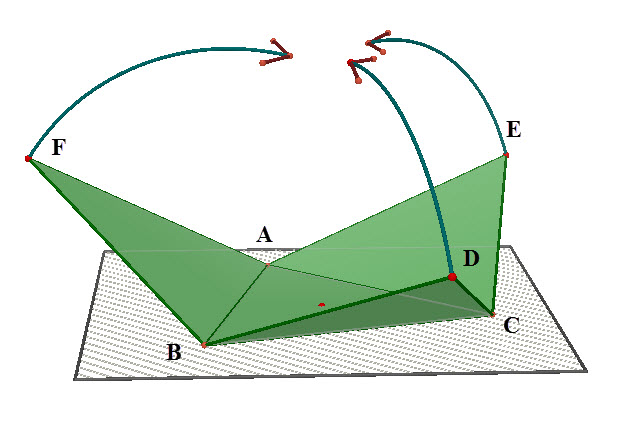
\includegraphics[width=\linewidth]{img/dichtplooien2.jpg}
\captionof{figure}{Simplex: van 2D naar 3D}
\label{dichtplooien2}
\end{center}

Maar hoe ziet een Platlander deze beweging? Die ziet de scharnierbeweging zoals wij ze zien in bovenaanzicht. De punten $D$, $E$ en $F$ komen naar elkaar toe in een inwendig punt van de driehoek $ABC$. In figuur \ref{dichtplooien3} zie je een tussenfase waarin de punten $D$, $E$ en $F$ elkaar nog net niet ontmoeten.

Tijdens het naar elkaar toekomen van de punten $D$, $E$ en $F$ zien de platlanders ook drie driehoeken die geleidelijk van vorm veranderen. Het lijkt alsof ze elastisch zijn. In de laatste fase rekken de driehoeken in de hoogte uit tot hun toppen elkaar raken.

\begin{center}
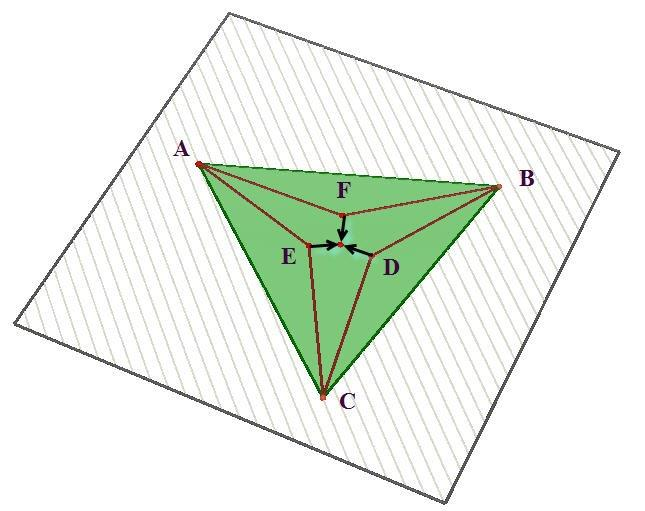
\includegraphics[width=\linewidth]{img/dichtplooien3.jpg}
\captionof{figure}{Bekeken door de bril van een platlander}
\label{dichtplooien3}
\end{center}

De derde stap is iets moeilijker in te beelden. Neem een regelmatig viervlak. Kleef aan de zijvlakken vier congruente viervlakken, zie figuur \ref{dichtplooien4}. Bed de driedimensionale ruimte in een vierdimensionale in en scharnier vervolgens de vier omringende viervlakken rond de zijvlakken van het centrale viervlak tot de toppen samenvallen. 

\begin{center}
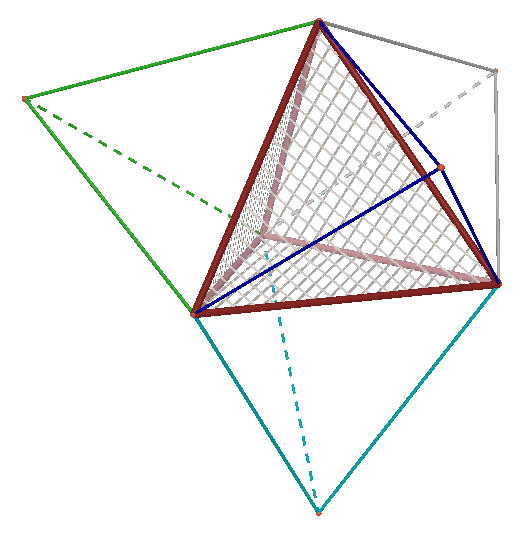
\includegraphics[width=\linewidth]{img/dichtplooien4.jpg}
\captionof{figure}{Simplex: van 3D naar 4D}
\label{dichtplooien4}
\end{center}

Wij, driedimensionale wezens, kunnen ons niet inbeelden hoe dit werkt, tenzij met een kunstgreep. Beeld je je het ruimtelichaam uit figuur \ref{dichtplooien4} in alsof het gemaakt is in een superelastisch materiaal. Dan is het wel mogelijk om de toppen naar elkaar toe te trekken tot ze elkaar raken. We hebben dan hetzelfde gevoel als de platlanders die zich een driedimensionale simplex proberen in te beelden.

Bij de beschrijving van het dichtvouwen doen we een sterk beroep op je verbeeldingskracht. Je trekt de toppen $E$, $F$, $G$ en $H$ van de omringende viervlakken naar elkaar toe en identificeert ze met een inwendig punt van het oorspronkelijke viervlak. Hierdoor zullen ook de ribben van de omringende viervlakken drie aan drie met elkaar geïdentificeerd worden, bijvoorbeeld $[DG]$, $[DE]$ en $[DF]$. Eveneens zullen de zijvlakken van de omringende viervlakken twee aan twee geïdentificeerd worden, bijvoorbeeld driehoek $BDG$ en driehoek $BDE$.

\begin{center}
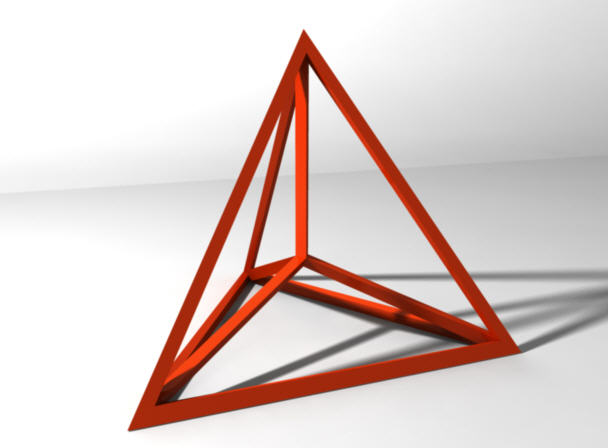
\includegraphics[width=\linewidth]{img/turbosquid.jpg}
\captionof{figure}{Een 4-simplex, in 3D geprint door \url{https://www.turbosquid.com/3d-models/tetrahedron-print-3d-model/864861}}
\label{turbosquid}
\end{center}

Het vierdimensionaal lichaam dat op deze manier ontstaat, is op veel plaatsen als tweedimensionale afbeelding terug te vinden op het internet. Ook driedimensionale afbeeldingen bestaan. Je kunt ze bestellen in gespecialiseerde 3D-printshops, zie figuur \ref{turbosquid}.

Een andere naam voor het vierdimensionale simplex is de \emph{vijfcel}. Als je figuur \ref{turbosquid} voor de eerste keer bekijkt, is de kans groot dat je maar vier cellen (in de vorm van een tetraëder) kunt onderscheiden. Het zijn de vier cellen die met een top in het centrum samenkomen. Maar er is er nog eentje, de grote tetraëder die de andere vier (in de driedimensionale perspectiefvoorstelling) verpakt.

\newpage

\end{multicols}
\begin{tabular}{|c|cccccc|}
  \hline
  \begin{tabular}[t]{@{}lr@{}}
           & Elementen: \\
    Dimensie: &
  \end{tabular}  & hoekpunten & ribben & driehoeken & tetraëders & 4-simplexen & 5-simplexen \\
  \hline
  0  &1   &0  &0   &0     &0     &0  \\
  1  &2   &1  &0   &0     &0     &0  \\
  2  &3   &3  &1   &0     &0     &0  \\
  3  &4   &6  &4   &1     &0     &0  \\
  4  &5   &10  &10   &5    &1     &0  \\
  5  &6   &15  &20   &15    &6   &1  \\
  6  &7   &21 &35  &35   &21    &7  \\
  \hline
\end{tabular}
\captionof{figure}{Overzicht van aantal elementen in een n-simplex}

\begin{multicols}{2}

\setlength{\parskip}{1em}
\tussentitel{Tellen van deelobjecten}

Bij het tellen van de deelobjecten van hogerdimensionale hyperkubussen, konden we terugvallen op een Pascalachtige driehoek, waarin we na enkele lijnen beredeneerd te hebben een duidelijk systeem zagen. Ook bij het tellen van de deelobjecten van hogerdimensionale simplexen is zulke werkwijze mogelijk. Om dit duidelijk te maken, tellen we eerst de deelobjecten van het 4-simplex.

Het 4-simplex ontstaat uit het 3-simplex door 1 hoekpunt toe te voegen. In de voorgaande beschouwing namen we een inwendig punt als extra hoekpunt. Het 4-simplex heeft dus 5 hoekpunten. Telkens wanneer we overstappen naar een simplex in de ruimte waarvan de dimensie met 1 vergroot, zal het simplex 1 hoekpunt bij krijgen. Dit onthouden we voor de opstelling van het Pascalachtige overzicht.

Kijken we nu even naar de ribben van het 4-simplex. Van deze ribben zijn er 6 overgeërfd van het oorspronkelijke 3-simplex. In elk hoekpunt van dit 3-simplex komen er nog eens drie ribben bij, die door identificatie overgaan in 1 enkele ribbe. Er komen dus nog 4 extra ribben bij. Het aantal ribben van het 4-simplex is bijgevolg gelijk aan 10. Dit is het aantal ribben van het 3-simplex vermeerderd met het aantal hoekpunten van het 3-simplex. We onthouden ook deze manier van tellen.

Vervolgens tellen we de driehoeken. Er waren er al 4 in het 3-simplex. Maar op elk van de 6 ribben kwamen er nog twee bij die telkens geïdentificeerd werden tot 1 driehoek. Samengevat: er zijn 4+6 driehoeken te vinden in een 4-simplex. Dit is de som van het aantal driehoeken van het 3-simplex en het aantal ribben van het 3-simplex.

En tot slot: hoeveel 3-simplexen zitten er in een 4-simplex. In figuur \ref{dichtplooien4} zie je 1 centraal 3-simplex waarbij op elk van de 4 zijvlakken er een nieuw 3-simplex is gekleefd. In totaal zijn er 5. Dit aantal is weer een som: het oorspronkelijke aantal 3-simplexen plus het aantal zijvlakken ervan.

Met deze kennis kunnen we de vijfde rij van de  tabel (figuur 21) invullen. Maar ook de rest van de tabel voldoet aan de regelmaat die we ontdekten.

Waarschijnlijk merk je meteen op dat deze Pascalachtige driehoek de echte driehoek van Pascal is. Elk getal is de som van de bovenbuur en de linkerbovenbuur. En als je uiterst links een kolom met eentjes toevoegt, dan komen ook de getallen aan de rand van de driehoek overeen met die van Pascal. Zo wordt de link met de combinatoriek duidelijk.


Het is dan ook niet meer nodig om een hele tabel uit te schrijven om bijvoorbeeld te berekenen hoeveel 3-simplexen er zitten in een 6-simplex. Je berekent dit meteen met de formule $C_7^3=35$. En als je wilt weten hoeveel 4-simplexen er zitten in een 9-simplex dan bereken je $C_{10}^4=210$.



\subsection{De vierdimensionale kubus, de vierdimensionale octaëder en meer van dat}

Na het voorbeeld van de aaneengekleefde tetraëders, vraag ik mijn leerlingen soms hoeveel kubussen ik elastisch aan elkaar moet kleven opdat elk vierkant zijvlak van een kubus zou kunnen grenzen aan een vierkant zijvlak van een andere kubus. Meestal vinden ze het antwoord. Het zijn er acht. Een tesseract of een vierdimensionale kubus bestaat uit acht kubusvormige cellen. De meest populaire voorstellingswijze van de tesseract zie je in figuur \ref{tesseract}. De afbeelding kun je vergelijken met twee verbonden kubussen in centraalperspectief. De grote kubus staat dichtbij, de kleinere verderaf.

Er zijn ook animaties op het internet te vinden van het elastisch samenvouwen van acht kubussen tot een tesseract. Eentje vind je op de website van Union College.

\begin{center}
\includegraphics[width=0.8\linewidth]{img/tesseract.png}
\captionof{figure}{De tesseract in centraalperspectief \\ (\url{https://nl.wiktionary.org/wiki/tesseract})}
\label{tesseract}
\end{center}



We stelden al twee regelmatige veelcellen of \emph{polytopen} in de vierdimensionale ruimte aan u voor: de regelmatige vijfcel en de regelmatige achtcel. 

\begin{center}
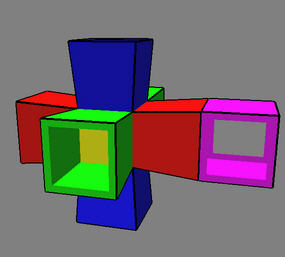
\includegraphics[width=\linewidth]{img/tesseractplooien.jpg}
\captionof{figure}{Samenvouwen van kubussen (\url{http://www.math.union.edu/~dpvc/math/4D/folding/hcube-folding.html})}
\label{tesseractplooien}
\end{center}

Regelmatige vierdimensionale polytopen zijn samenkleefsels van een aantal congruente regelmatige veelvlakken. In elk hoekpunt moeten ze ook met evenveel samenkomen. 

Het is bekend hoeveel regelmatige polytopen er nog zijn in vier dimensies. Het zijn er zes. Naast de vijfcel en de achtcel zijn er: de 16-cel die bestaat uit 16 tetraëders, de 24-cel die bestaat uit 24 octaëders, de 120-cel die bestaat uit 120 dodecaëders en de 600-cel die bestaat uit 600 tetraëders. 

Ook in hogerdimensionale ruimten is het aantal regelmatige polytopen gekend. In elke dimensie hoger dan vier is dit aantal 3. Fascinerend maar we zullen hier niet dieper op ingaan.

Hoe de 24-cel wordt opgebouwd, kunnen we wel laten zien. Hiervoor hebben we een zeer kort YouTube-filmpje gemaakt. Het laat zien hoe je twee conglomeraten van 9 octaëders aan elkaar kunt zetten met 6 extra octaëders. Als alle onderdelen samengekleefd zijn, grenst elk zijvlak aan precies twee octaëders. De constructie mag dan als \emph{gesloten} beschouwd worden.

\begin{center}
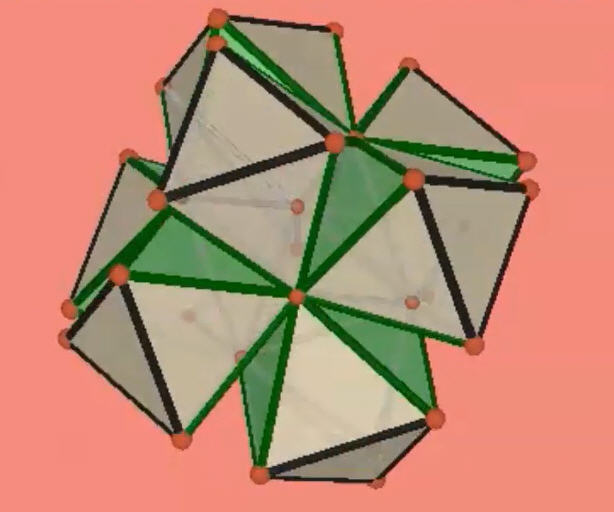
\includegraphics[width=\linewidth]{img/4d_octaeder.jpg}
\captionof{figure}{De constructie van de vierdimensionale octaëder (\url{https://www.youtube.com/watch?v=6gDCIrJSZ6g})}
\label{4d_octaeder}
\end{center}

Heb je wat meer tijd in de klas, dan is het YouTube-filmpje \emph{Perfect Shapes in Higher Dimensions} een aanrader. Hierin wordt het bewijs gegeven dat er slechts zes regelmatige polytopen zijn in de vierdimensionale ruimte. Ze worden een voor een opgebouwd en getoond, tot zelfs de 120-cel en de 600-cel toe.

\begin{center}
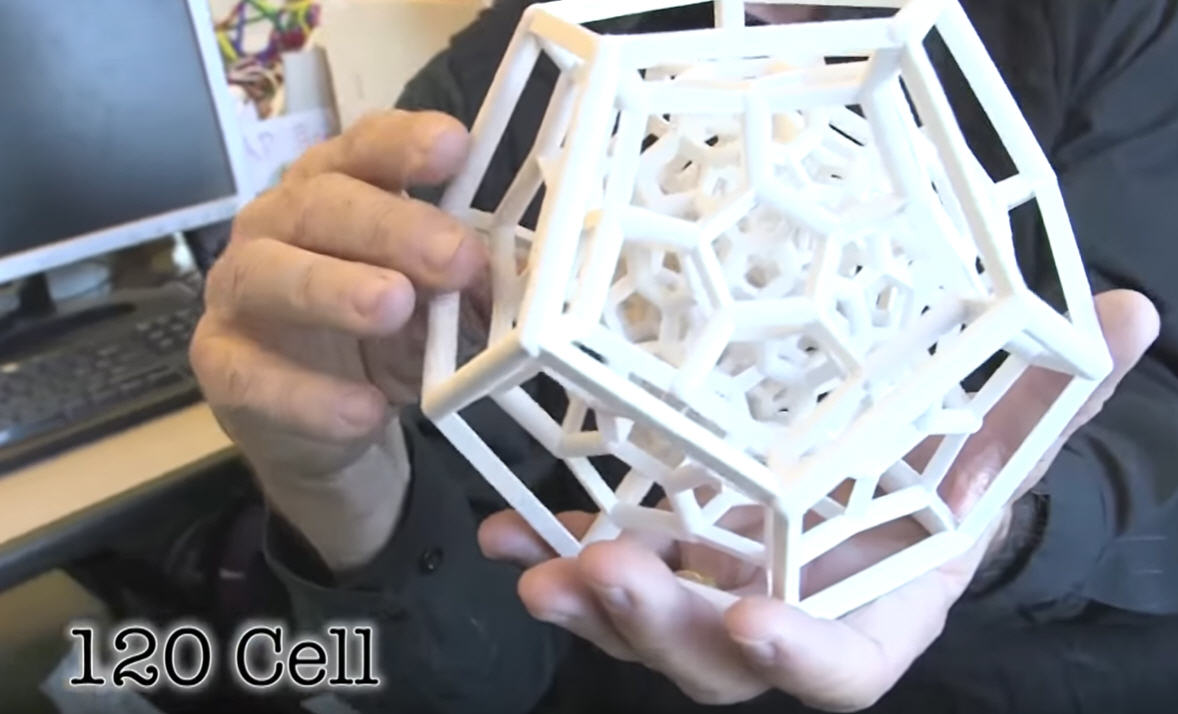
\includegraphics[width=\linewidth]{img/120cel.jpg}
\captionof{figure}{De 120-cel (https://www.youtube.com/watch?v=2s4TqVAbfz4)}
\label{120cel}
\end{center}

Het nadenken over de visuele voorstelling van vierdimensionale lichamen hoort niet bij een of ander onderdeel van de leerstof van het secundair onderwijs. Toch is het iets wat leeft bij sommige leerlingen. Uit eigen ervaring weet ik dat het tonen van dit en soortgelijk materiaal verwondering wekt en dat de vierde dimensie hierdoor een boogscheut dichterbij komt.

\section{Rekenen met coördinaten}

Rekenen met coördinaten is een beproefde methode om meetkunde te bedrijven zonder dat het meetkundige inzicht allesbepalend is. Wanneer we een meetkundig bewijs moeten geven en we vinden niet meteen de juiste synthetische argumenten, dan grijpen we wel vaker naar een analytische aanpak met coördinaten en vergelijkingen.

Het ruimtelijk inzicht in de vierdimensionale en hogerdimensionale meetkunde is zeer moeizaam te verwerven, zelfs bij geroutineerde wiskundigen. Daarom wordt het des te interessanter meetkundige problemen te vertalen naar algebraïsche berekeningen. We rekenen immers bijna net zo vlot met viertallen of vijftallen als met tweetallen en drietallen. 

De formules die we in hogere dimensies gebruiken, kunnen vaak ook met weinig moeite afgeleid worden uit de formules in lagere dimensies. Denken we bijvoorbeeld aan de formule voor de afstand tussen twee punten of de formule voor het zwaartepunt van een simplex. Over deze twee formules hebben we het verderop nog. De eerste formule zullen we vanuit de coördinatenmeetkunde belichten, de tweede vanuit het vectorrekenen.

\subsection{De formule voor de euclidische afstand}

Beeld je in dat we de afstand tussen de punten $P(x_1, y_1, z_1)$ en $Q(x_2, y_2, z_2)$ in de driedimensionale ruimte willen berekenen en dat we enkel kunnen terugvallen op de afstandsformule in de tweedimensionale ruimte. Dan kunnen we dit voor elkaar krijgen door twee afstandsberekeningen aan elkaar te koppelen.

Bereken eerst de afstand tussen de hulppunten $P'(x_1, y_1, 0)$ en $Q'(x_2, y_2, 0)$ in het $xy$-vlak. Hiervoor gebruiken we de formule $\sqrt{(x_2-x_1)^2+(y_2-y_1)^2}$, die rechtstreeks volgt uit de stelling van Pythagoras. 

Omdat de richting van de $z$-as loodrecht staat op het $xy$-vlak, kunnen we de stelling van Pythagoras een tweede keer toepassen. We gebruiken de stelling ditmaal in een rechthoekige driehoek met als schuine zijde $[PQ]$ en met rechthoekszijden evenwijdig met de $z$-as en met het $xy$-vlak. 

De lengten van de rechthoekszijden zijn $\sqrt{(x_2-x_1)^2+(y_2-y_1)^2}$ en $\abs{z_2-z_1}$. De lengte van de schuine zijde $\abs{PQ}$ is bijgevolg gelijk aan:
\[ \sqrt{(x_2-x_1)^2+(y_2-y_1)^2+(z_2-z_1)^2}.\]

\begin{center}
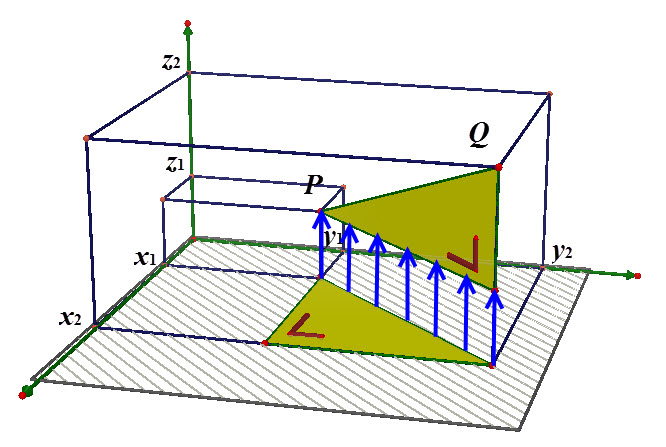
\includegraphics[width=\linewidth]{img/tweekeerpythagoras.jpg}
\captionof{figure}{Afstandsformule: van 2D naar 3D}
\label{tweekeerpythagoras}
\end{center}

Deze redenering kunnen we op een technische manier verderzetten naar hogere dimensies. 

Stel dat we de afstand moeten berekenen tussen de vierdimensionale punten $P(x_1, y_1, z_1, t_1)$ en $Q(x_2, y_2, z_2, t_2)$ en we kunnen enkel steunen op een afstandsformule in een driedimensionale ruimte dan construeren we de hulppunten $P'(x_1, y_1, z_1, 0)$ en $Q'(x_2, y_2, z_2, 0)$. De afstand tussen deze punten is gelijk aan $\sqrt{(x_2-x_1)^2+(y_2-y_1)^2+(z_2-z_1)^2}$.

Aangezien we nog een tweede keer op de stelling van Pythagoras willen steunen, zullen we de $t$-as nu ook loodrecht op de $x$-as, de $y$-as en de $z$-as moeten plaatsen, m.a.w. op de $xyz$-ruimte. In een vierdimensionale ruimte lukt dit. 

We beschouwen nu de rechthoekige driehoek met als schuine zijde het lijnstuk $[PQ]$, met een rechthoekszijde evenwijdig met de $t$-as en de andere in de $xyz$-ruimte. De lengten van de rechthoekszijden zijn $\abs{t_2-t_1}$ en $\sqrt{(x_2-x_1)^2+(y_2-y_1)^2+(z_2-z_1)^2}$. Bijgevolg is de schuine zijde $\abs{PQ}$ gelijk aan:
\[ \sqrt{(x_2-x_1)^2+(y_2-y_1)^2+(z_2-z_1)^2+(t_2-t_1)^2}.\]

Deze redenering die stapsgewijze opklimt naar ruimten met een hogere dimensie, kan nu moeiteloos verder gezet worden om de afstandsformule te ontwikkelen tussen twee punten in een vijfdimensionale, een zesdimensionale, ... ruimte.

\subsection{Een diameter van een hyperkubus}

Onder de \emph{diameter} van een veelhoek, een veelvlak of een polytoop, verstaan we (net zoals bij cirkels) de langste afstand tussen twee hoekpunten van deze veelhoek, dit veelvlak of deze polytoop. We kunnen ook spreken van de lengte van de langste diagonaal. 

Nu de afstandsformule in een ruimte van een willekeurige dimensie gekend is, kunnen we de diameter berekenen van een willekeurige hyperkubus. Bij wijze van voorbeeld zullen we de diameter van een vierdimensionale eenheidskubus of de tesseract met ribbe 1 berekenen. 

In een vorige paragraaf lieten we zien dat deze tesseract 16 hoekpunten heeft. De coördinaten van de hoekpunten van de tesseract die ontstond door een gewone kubus te verschuiven in de vierde dimensie, somden we op in figuur \ref{fig13}. We noteren deze coördinaten ook nog een keer bij de andere visuele voorstelling van de tesseract, die te zien is in figuur \ref{langstediagonaal}.

\begin{center}
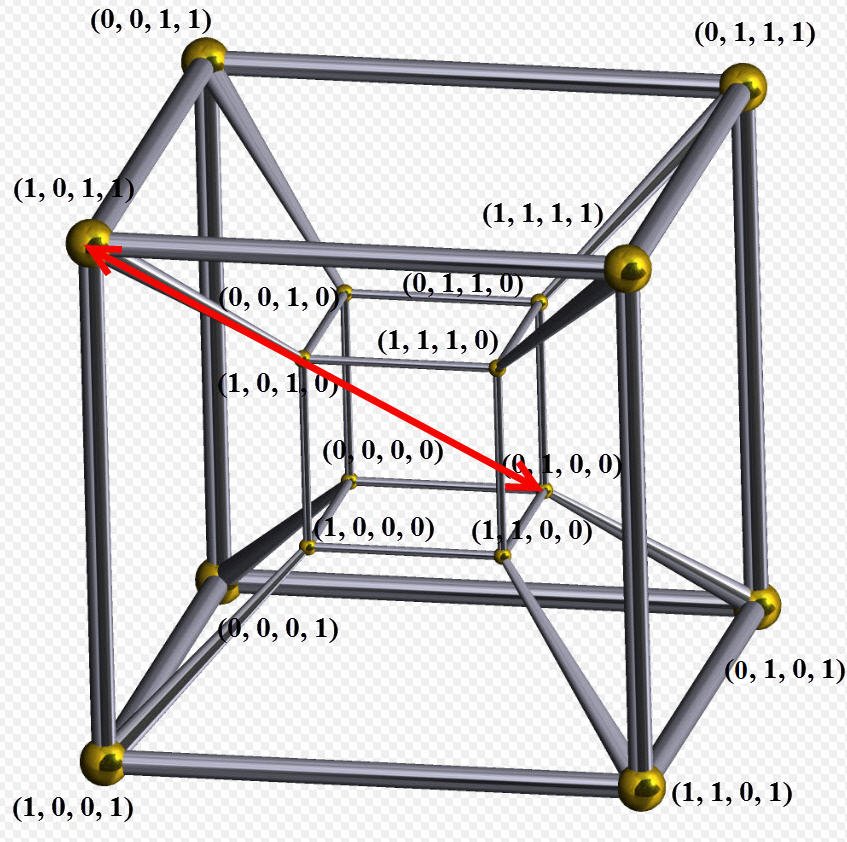
\includegraphics[width=\linewidth]{img/delangstediagonaal.jpg}
\captionof{figure}{Een langste diagonaal van de tesseract}
\label{langstediagonaal}
\end{center}

De lengte van een langste diagonaal vinden we door twee hoekpunten van de tesseract te verbinden die niet op eenzelfde ribbe liggen, niet op eenzelfde zijvlak en niet in eenzelfde driedimensionale (vervormde) kubus. In figuur \ref{langstediagonaal} is één langste diagonaal aangeduid maar er zijn nog zeven andere mogelijkheden. De keuze viel op het lijnstuk dat de punten $(1, 0, 1, 1)$ verbindt met het punt $(0, 1, 0, 0)$. Het zal je misschien verbazen dat deze \emph{overhoekse} diagonaal een gehele lengte heeft:
\[ \sqrt{\left(1-0\right)^2+\left(0-1\right)^2+\left(1-0\right)^2+\left(1-0\right)^2}=2.\]

Er zijn ook nog andere hyperkubussen met zijde 1 die een diameter hebben met een geheel maatgetal. Denk maar aan de hyperkubus in de negendimensionale ruimte als je je die kunt voorstellen. De acht overhoekse diagonalen van de tesseract snijden elkaar middendoor. Hun snijpunt is het punt $M\left( \frac{1}{2}, \frac{1}{2}, \frac{1}{2}, \frac{1}{2}\right)$. Dit punt ligt op gelijke afstand van de 16 punten van de tesseract. We rekenen één van deze afstanden uit:

\[ \sqrt{\left(1-\frac{1}{2}\right)^2+\left(1-\frac{1}{2}\right)^2+\left(0-\frac{1}{2}\right)^2+\left(1-\frac{1}{2}\right)^2}=1.\]

Hiermee hebben we meteen aangetoond dat de tesseract met ribbe 1 een omgeschreven bol heeft met straal 1. Of liever: een omgeschreven \emph{hyperbol}, een bol in een hogerdimensionale ruimte.

\subsection{De paradox van het opgesloten bolletje}

Dat het aantal hoekpunten van een $n$-dimensionale kubus aangroeit volgens de exponentiële functie $f(n)=2^n$ is zeer begrijpelijk. Dat de diameter van een $n$-dimensionale eenheidskubus groter wordt bij toenemende dimensies is ook niet tegenintuïtief. De diagonaal groeit aan volgens de wortelfunctie $f(n)=\sqrt{n}$. 

Deze twee uitspraken over meerdimensionale kubussen liggen binnen het verwachtingspatroon. Maar er is een bizar contrast tussen het exponentieel aangroeien en de aangroei volgens een machtsfunctie. Dit moet tot een paradox leiden ... 

Hieronder een probleem dat je aan het denken kan zetten. Als je jezelf de kans wilt geven om er op eigen kracht uit te raken, lees dan niet verder dan de ingesprongen tekst. 

\begin{citaat} {De $2^n$ hoekpunten van een $n$-dimensionale (hyper)kubus met ribbe 1 worden gebruikt als middelpunten van $2^n$ congruente (hyper)bollen die elkaar raken in de middens van de ribben. 

In de holle ruimte tussen al deze (hyper)bollen wordt een klein (hyper)bolletje opgesloten dat precies aan elk van deze (hyper)bollen raakt. Bepaal de functie $f(n)$ die de diameter van het opgesloten (hyper)bolletje weergeeft. 

Kan de diameter van het opgesloten (hyper)bolletje groter zijn dan 1? Wat besluit je hier uit? } 
\end{citaat}

In figuur \ref{ingeslotencirkel} zie je het opgesloten bolletje in een 'tweedimensionale kubus'. Het centrale bolletje is relatief klein ten opzichte van de omringende bollen. In figuur \ref{ingeslotenbolletje} zie je iets gelijkaardigs in een driedimensionale kubus. Het ingesloten bolletje lijkt iets groter ten opzichte van de omringende bollen. Maar dat kan ook gezichtsbedrog zijn. 

In beide gevallen zitten de centrale bolletjes niet alleen netjes opgesloten tussen de omringende bollen, ze zitten ook gevangen in de eenheidskubus. Om hier absoluut zeker van te zijn, moeten we de diameter van dit bolletje berekenen.

\begin{center}
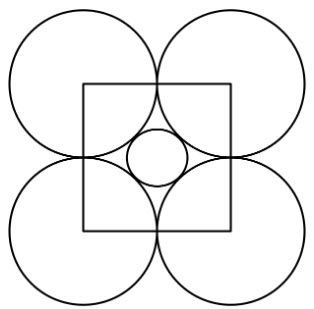
\includegraphics[width=0.75\linewidth]{img/ingeslotencirkel.jpg}
\captionof{figure}{Het opgesloten bolletje in twee dimensies}
\label{ingeslotencirkel}
\end{center}

\begin{center}
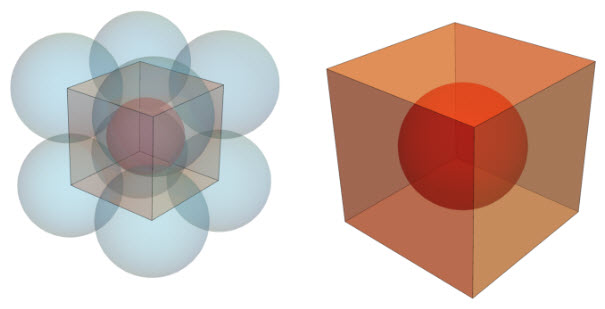
\includegraphics[width=\linewidth]{img/ingeslotenbolletje.jpg}
\captionof{figure}{Het opgesloten bolletje in drie dimensies (\url{https://marckhoury.github.io/counterintuitive-properties-of-high-dimensional-space/})}
\label{ingeslotenbolletje}
\end{center}

De overhoekse diagonaal van de tweedimensionale eenheidskubus heeft een lengte gelijk aan $\sqrt{2}$. We vinden de diameter $d$ van het ingesloten bolletje door twee keer de straal van de omringende bollen van deze lengte af te trekken:
\[d= \sqrt{2} -2 \cdot \frac{1}{2}= \sqrt{2}-1=0,41 \dots\]

De lengte van de overhoekse diagonaal van een driedimensionale eenheidskubus is $\sqrt{3}$. Analoog vinden we dan dat:
\[d= \sqrt{3} -2 \cdot \frac{1}{2}= \sqrt{3}-1=0,73 \dots\]

Het centrale bolletje wordt inderdaad groter als de dimensie verhoogt van 2 naar 3. Maar het puilt in deze voorbeelden nog niet door de zijvlakken van de kubus. Daarvoor moet de diameter groter dan 1 zijn.

Vanaf dimensie 5 breekt het kleine bolletje tegen de intuïtie in door de zijvlakken van de hyperkubus. De diameter is dan groter dan 1:
\[d= \sqrt{5} -2 \cdot \frac{1}{2}= \sqrt{5}-1=1,23 \dots\]

Er zijn nog meer paradoxen bekend in verband met de hyperkubussen met ribbe 1. De inhoud van een eenheidshyperkubus in een ruimte van een willekeurige dimensie is gelijk aan 1. Maar de diagonaal kan zo groot worden als je maar wilt.

Stel nu dat er een buitenaards wezen vanuit een $n$-dimensionaal universum met malafide bedoelingen naar ons universum komt. Dan zou deze alien een klein eenheidshyperkubusje van $1 \times 1 \times 1 \times \cdots \times 1$ cm$^n$ pervers kunnen inzetten bij een geslaagde kunstroof. Voor zeer grote $n$ past de Eiffeltoren immers netjes in de diagonaal in deze hyperkubus. En de hyperkubus met een inhoud van 1 cm$^n$ past dan weer precies in de binnenzak van de alien. De perfecte misdaad?


\subsection{De inhoud van bollen in hogere dimensies}

Een van de leukste ongeloofwaardigheden betreft de inhoud van de hyper-bol (ik schrijf het even met een koppelteken om de verwarring met hyperbool te vermijden) met straal 1. Wanneer we deze inhoud berekenen in ruimten met dimensies die opklimmen van 1 tot 5, blijkt die alsmaar groter te worden. De eenheidshyperbol in de vijfdimensionale ruimte heeft een maximale inhoud, gelijk aan $\frac{8 \pi^2}{15}$. Vanaf de ruimte met dimensie 6 neemt deze inhoud alleen nog maar af. 

Nog gekker is het gesteld met de oppervlakten van eenheidshyperbollen. Die nemen toe tot en met dimensie 7 en daarna nemen ze weer af. De oppervlakte van een zevendimensionale eenheidshyperbol is $\frac{16 \pi^3}{15}$. 

De exacte afleiding van de formule voor de inhouden van $n$-dimensionale eenheidsbollen is geen onderzoeksdomein dat geschikt is voor onze leerlingen. Maar deze inhoud tot op enkele cijfers na de komma benaderen, kan heel goed in de klas. Op deze manier kunnen leerlingen toch merken dat het na de vijfde dimensie achteruit gaat met de inhoud.

We illustreren de werkwijze voor dimensie 4. Plaats een vierdimensionale bol met straal 1 met het middelpunt in de oorsprong $(0, 0, 0, 0)$. Teken in gedachte een vierdimensionale kubus rond deze bol. Neem daarna een zeer groot aantal willekeurige punten uit deze kubus, m.a.w. uit $[-1,1]\times[-1,1]\times[-1,1]\times[-1,1]$. Indien de afstand van een van deze punten tot $(0, 0, 0, 0)$ kleiner is dan 1 dan ligt dit punt in de eenheidshyperbol. De relatieve frequentie van de punten uit de hyperkubus die in de eenheidsbol liggen (of de kans dat een punt hierin ligt) kan berekend worden door een computersimulatie te doen. Vermenigvuldig deze kans met de inhoud van de hyperkubus ($2^4$) en je vindt de inhoud van de eenheidsbol. 

Als je deze simulatie wilt doen en je wilt de looptijd van het programma beperken tot maximaal één lesuur, dan moet je je grafische zakrekenmachine achterwege laten. Je hebt dan immers een supersnelle rekenaar nodig. Zelf heb ik een gratis account gemaakt van CoCalc (\url{https://cocalc.com/}) waarin ik programmeer met de programmeertaal Sage, die erg verwant is met Python. In figuur \ref{programma} zie je een kort programma dat je gewoon in CoCalc kan overnemen. We zetten het op onze website.


Wie gewoon is om programmacode te lezen, neemt deze regels door als een krantenartikel. Maar voor de meeste leerlingen zal hier een woordje uitleg noodzakelijk zijn. De functie \emph{binnen}() kiest een willekeurig punt uit de omgeschreven hyperkubus en onderzoekt of dit punt binnen de eenheidshyperbol ligt. \emph{Binnen}() geeft $R=1$ als output bij succes en $R=0$ bij een mislukking. De functie \emph{kansbinnen}() kiest 10 miljoen van deze punten en telt de relatieve frequentie dat ze binnen liggen. Voor 10 miljoen van deze punten had ik een tiental minuten geduld nodig. 

Het resultaat van deze simulatie was een inhoud gelijk aan $4,93...$ die op twee cijfers na de komma overeenkomt met de theoretische inhoud van de vierdimensionale eenheidshyperbol ($\frac{\pi^2}{2}$). 

Op deze manier is het technisch goed mogelijk een onderzoek te doen naar de inhouden van de eenheidsbollen in alle mogelijke dimensies en zich op deze manier te laten verwonderen over de bol in de vijfdimensionale ruimte.

\end{multicols}
\begin{center}
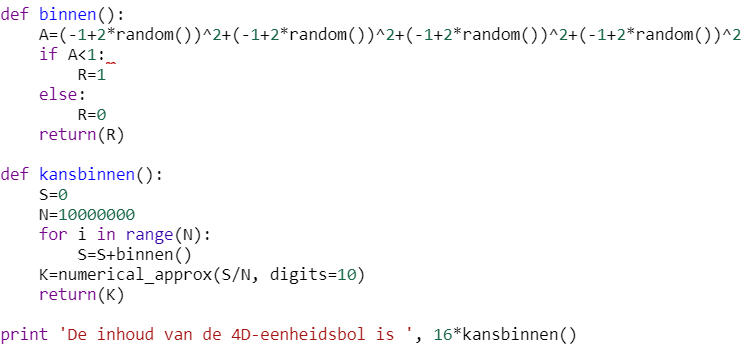
\includegraphics[width=0.9\linewidth]{img/programma.jpg}
\captionof{figure}{Een programma in CoCalc}
\label{programma}
\end{center}
\begin{multicols}{2}
\setlength{\parskip}{1em}

\subsection{De formule voor de Hamming-afstand}

Naast de euclidische afstandsformule bestaat nog een andere, die minstens even belangrijk is in de hogerdimensionale meetkunde, de Hamming-afstand. Ze wordt toegepast op een binaire ruimte. Hiermee bedoelen we een verzameling van $n$-tallen waarbij elk coördinaatgetal ofwel 1 ofwel 0 is. De $n$-tallen van de vorm $(a_1, a_2, a_3, ... a_n)$ waarbij $a_i \in \{0, 1\}$ stellen de hoekpunten voor van een $n$-dimensionale kubus. 


In figuur \ref{vijfdimensionalekubus} zie je een vijfdimensionale kubus. Hij is opgebouwd via de verschuivingsmethode, die we eerder al ter sprake brachten. De 32 hoekpunten van deze hyperkubus worden aangeduid met 32 verschillende vijftallen. 

De Hamming-afstand tussen twee hoekpunten van de hyperkubus wordt gegeven door de formule 
\[d_H((a_1, a_2, ... a_n), (b_1, b_2, ... b_n))= \sum\limits_{i=1}^{n} \abs{a_i-b_i}.\]
In gewone taal zeggen we dat de Hamming-afstand tussen twee punten gelijk is aan het aantal ribben van de hyperkubus dat minimaal moet gebruikt worden om van het ene punt naar het andere te wandelen. In andere contexten wordt deze afstand de \emph{taxi-afstand} genoemd. We kunnen ook zeggen dat de Hamming-afstand gelijk is aan het aantal posities waarin de coördinaten van de twee punten verschillen.

De langste diagonaal van de hyperkubus in figuur \ref{vijfdimensionalekubus} heeft Hamming-lengte 5:
\[d_H((0, 1, 1, 0, 0), (1, 0, 0, 1, 1))\] 
\[= \abs{0-1}+\abs{1-0}+\abs{1-0}+\abs{0-1}+\abs{0-1}=5.\]

Hamming-afstanden hebben hun belang in de codetheorie. Stel dat je 32 letters in een alfabet hebt en dat je deze letters moet omzetten in enen en nullen om ze digitaal te kunnen verzenden, dan kun je hiervoor gebruik maken van de hoekpunten van een vijfdimensionale kubus. Wij hebben slechts 26 letters in ons alfabet. Indien we dit zouden uitbreiden met een zestal leestekens en accenten, zou een code in een vijfdimensionale ruimte misschien net volstaan.

\tussentitel{Foutdetectie}

Echter, elke digitale verzending van gegevens houdt een mogelijkheid op een transmissiefout in, hoe klein ook. In de codetheorie houdt men er rekening mee dat één van de coördinaatgetallen van een gecodeerde letter kan verspringen. Er wordt nauwelijks rekening gehouden met de verspringing van twee van deze coördinaatgetallen. Die kans is klein-in-het-kwadraat, heel erg klein dus.

\end{multicols}

\begin{center}
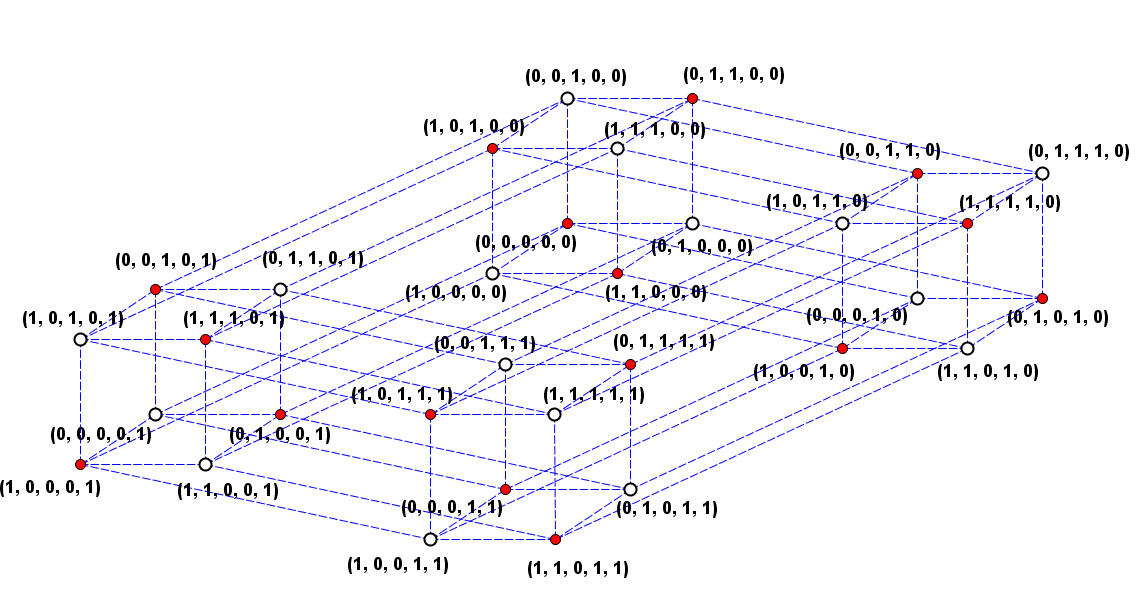
\includegraphics[width=\linewidth]{img/vijfdimensionalekubus.jpg}
\captionof{figure}{Coderen in een vijfdimensionale kubus}
\label{vijfdimensionalekubus}
\end{center}

\begin{multicols}{2}
\setlength{\parskip}{1em}

Als een coördinaatgetal bij de verzending verspringt, zal een bepaalde letter vervangen worden door een andere letter die overeenkomt met een aangrenzend hoekpunt van de hyperkubus. Dit kan voor verwarring zorgen. Als de I bijvoorbeeld naast de J ligt, dan kan het woord \emph{beiaard} per ongeluk omgezet worden in \emph{bejaard}. Vaak zul je een dergelijke fout opmerken omdat bepaalde woorden niet binnen de context passen maar het is beter om ze automatisch te laten detecteren door gepaste software.

Daarom is het aangewezen om niet alle hoekpunten van de hyperkubus te associëren met een letter van het alfabet. Als we enkel de holle bolletjes op de hoekpunten van de kubus in figuur \ref{vijfdimensionalekubus} als een geldige letter gebruiken, dan vallen enkelvoudige verspringingen in de coördinaten meteen op. Het hoekpunt van de kubus dat een letter voorstelt, verspringt naar een naburig hoekpunt dat geen letter voorstelt. Met deze strategie blijven er nog 16 hoekpunten (letters) over. Deze letters zijn met te weinig om een willekeurige tekst in het Nederlands te kunnen omzetten. Maar ze hebben wel als voordeel dat elke enkelvoudige fout gedetecteerd kan worden. Voor een foutdetecterende code moet elke Hamming-afstand tussen twee geldige letters minstens gelijk zijn aan 2.

Even een voorbeeld. Als de letter $(0, 1, 1, 0 ,0)$ wordt ontvangen van een correspondent, dan weet je dat hier een fout in zit. Je ziet dit op figuur 31. Het corresponderende punt is immers geen hol bolletje. Je merkt dit ook, en sneller zelfs, doordat de som van de coördinaatgetallen even is. De fout is dus gedetecteerd. Maar ze kan niet nauwkeurig verbeterd worden. Er blijft immers twijfel uit vijf letters, die geassocieerd worden aan de vijf hoekpunten die grenzen aan $(0, 1, 1, 0 ,0)$.

\tussentitel{Foutcorrectie}

Om een fout te kunnen \emph{verbeteren} moet de Hamming-afstand tussen twee geldige letters minstens drie zijn. In figuur \ref{hammingkubus} zie je een codering in een driedimensionale kubus. Enkel de hoekpunten $(0, 0, 1)$ en $(1, 1, 0)$, aangeduid met holle bolletjes, vormen geldige letters. De afstand tussen deze letters is 3. Als er een transmissiefout optreedt, kan die makkelijk verbeterd worden. De transmissie $(0, 1, 1)$ stelt bijvoorbeeld geen letter voor. Er is slechts één geldige letter die grenst aan $(0, 1, 1)$, namelijk $(0, 0, 1)$. Hierdoor is een correctie van een enkelvoudige fout mogelijk.

Merk op dat foutverbeterende codes in staat zijn om enkelvoudige en dubbele transmissiefouten te detecteren. Als de afstand tussen twee geldige letters 3 is, zullen er geen geldige letters te vinden zijn op een afstand 2 of 1 van een geldige letter. 

\begin{center}
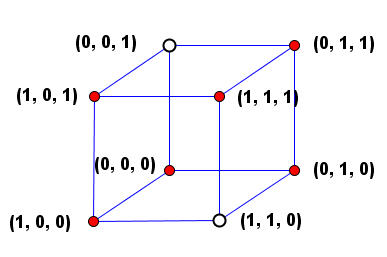
\includegraphics[width=0.8\linewidth]{img/hammingkubus.jpg}
\captionof{figure}{Coderen in een driedimensionale kubus}
\label{hammingkubus}
\end{center}

\tussentitel{Verdere problemen}

We kunnen ons nog enkele bijkomende vragen stellen. Hoeveel hoekpunten op een vijfdimensionale kubus kunnen we kleuren om een foutverbeterende code te maken? En: hoeveel dimensies hebben we minimaal nodig om de 26 letters van ons alfabet om te kunnen zetten in een foutverbeterende code? En: in welke dimensie bestaat er een foutverbeterende code waarbij de fractie van de hoekpunten die een geldige letter voorstellen, groter is dan bij andere dimensies?

Op deze vragen geven we geen antwoord in deze loep. We signaleren ze enkel om aan te tonen welk belang de $n$-dimensionale kubussen hebben bij het coderen. 

Tot slot merken we op dat de (7, 4)-Hamming-code een bijzondere rol inneemt. Op een 7-dimensionale kubus worden $2^4$ letters vastgelegd. De 16 letters van deze code zijn nog ruim onvoldoende om al onze letters en cijfers te coderen. Ook de (15, 11)-code wordt vaak gebruikt. Het aantal gecodeerde letters in dit systeem is dan weer ruim groot voor dagelijks gebruik. Als we alle letters, cijfers, leestekens, emoticons en wiskundesymbolen in een lijstje zouden zetten, komen we lang niet aan 2048 tekens.

\newpage

\section{Vectorrekenen in hogere dimensies}

In het zesde jaar vertrek ik in ruimtemeetkunde meestal vanuit vectoren en vectoriële vergelijkingen om daarna coördinaten en cartesiaanse vergelijkingen in te voeren. 

Ik start met het onderscheid tussen vrije vectoren, die met behoud van richting, lengte en zin door de ruimte rond kunnen vliegen, en gebonden vectoren, die met hun staartje vastgenageld zijn in de oorsprong. We kunnen vrije vectoren binden met de formule:
\[ \overrightarrow{AB}=\vec{B}-\vec{A}.\]

% Let op. Om de pijltjes boven de letters te krijgen moet de instructie \vec in de preamble aangepast worden door gebruik te maken van de instructie \overrightarrow.

Daarna volgen de definities van de vectorsom en het product van een vector met een getal samen met hun eigenschappen. Zowel de verzameling van de vrije vectoren als de verzameling van de gebonden vectoren vormt een vectorruimte wanneer ze uitgerust is met deze twee bewerkingen. Deze eigenschappen sommen we hier niet op. We gebruiken ze vrijuit in al wat volgt.

Het begrip lineaire onafhankelijkheid is niet makkelijk voor de leerlingen. De definitie \emph{geen van de vectoren kan geschreven worden als een lineaire combinatie van de overige verctoren} is begrijpbaar maar er valt moeilijk mee te rekenen. Daarom is er een praktische vertaling nodig, bijvoorbeeld: de vectoren $\vec{A}$, $\vec{B}$ en $\vec{C}$ zijn lineair onafhankelijk als en slechts als:
\[k \cdot \vec{A} + l \cdot \vec{B} + m \cdot \vec{C}= \vec{O} \quad \Rightarrow \quad k=l=m=0.\]
Dit betekent zoveel als: geen enkele lineaire combinatie van deze vectoren kan de nulvector opleveren tenzij de triviale lineaire combinatie (de lineaire combinatie met enkel 0 als coëfficiënten).

Tot slot komen we tot de vectoriële vergelijkingen van rechten en vlakken waarbij er een aantal punten en richtingsvectoren gegeven zijn. Zo leiden we bijvoorbeeld de vergelijking van de rechte af door twee niet samenvallende punten $A$ en $B$:
\[\vec{P}=(1-k) \vec{A} +k \vec{B}.\]

Het punt $P$ is een variabel punt op deze rechte en de parameter $k$ loopt van $-\infty$ tot $+\infty$ als het punt $P$ alle punten van de rechte doorloopt van de ene kant naar de andere kant, zo ver je je maar kunt indenken.

Met deze summiere basisformules kunnen heel wat interessante stellingen bewezen worden. Meer nog, bepaalde stellingen kunnen veralgemeend worden vanuit een rechte, naar een vlak, naar de driedimensionale ruimte en verder. Hieronder beschrijven we dit proces voor de berekening van zwaartepunten van een willekeurige simplex.

\subsection{Zwaartepunt van een lijnstuk}

Met het zwaartepunt van een lijnstuk bedoelen we het midden van dit lijnstuk. Bij lijnstukken kun je het zwaartepunt ook makkelijk fysisch interpreteren: als je een homogeen staafje in het midden ondersteunt dan blijft het in evenwicht balanceren.

Stel dat twee punten $A$ en $B$ of twee gebonden vectoren $\vec{A}$ en $\vec{B}$ gegeven zijn. Welke vectorbewerking moet je dan op deze vectoren uitvoeren om de gebonden vector $\vec{M}$ te vinden die geassocieerd wordt met het midden $M$ van het lijnstuk $[AB]$?

Voor problemen met zwaartepunten is het vaak overbodig om met coördinaten te werken. We laten in een serie opeenvolgende oefeningen zien dat vectoren hier krachtig genoeg zijn. 

\begin{center}
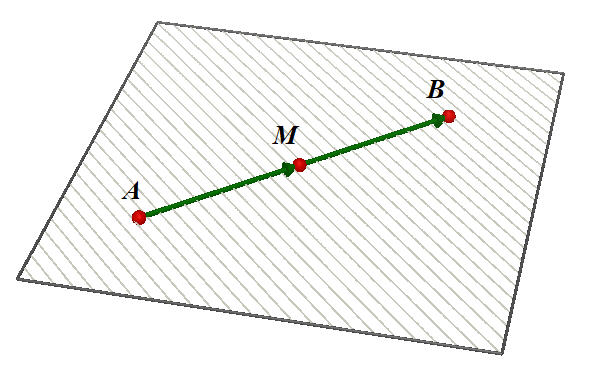
\includegraphics[width=\linewidth]{img/zwaartepunt1.jpg}
\captionof{figure}{Het zwaartepunt van een lijnstuk}
\label{zwaartepunt1}
\end{center}

Deze inleidende oefening op het begrip zwaartepunt is in enkele stappen opgelost. We gebruiken de definitie van het midden van een lijnstuk die steunt op vrije vectoren:
\[\vec{AM}=\vec{MB}\]
en zetten deze vrije vectoren meteen om naar gebonden vectoren:
\[\vec{M}-\vec{A}=\vec{B}-\vec{M}.\]

We zoeken nu een directe uitdrukking voor $\vec{M}$. In klassen die de vectorruimtestructuur behandeld hebben (bijvoorbeeld in het GO!) is het interessant te preciseren welke eigenschappen van de vectorruimte je hier achtereenvolgens voor nodig hebt. Maar dat doen we hier niet. Het resultaat van deze afleiding is:
\[\vec{M}=\frac{\vec{A}+\vec{B}}{2}.\]

De zwaartepuntsvector is het gemiddelde van de vectoren die geassocieerd zijn aan de eindpunten van het lijnstuk. 

We proberen nu een gelijkaardig resultaat af te leiden in de tweedimensionale ruimte.

\subsection{Zwaartepunt van een driehoek}

Het zwaartepunt van een driehoek is het snijpunt van de drie zwaartelijnen. Een zwaartelijn van een driehoek is een rechte die een hoekpunt met het zwaartepunt van de overstaande zijde verbindt. 

Deze twee definities leggen een verband tussen het zwaartepunt van een lijnstuk en het zwaartepunt van een driehoek. Op deze manier is het mogelijk om een vectoruitdrukking te vinden voor het zwaartepunt $Z$ van een willekeurige driehoek $ABC$.

\begin{center}
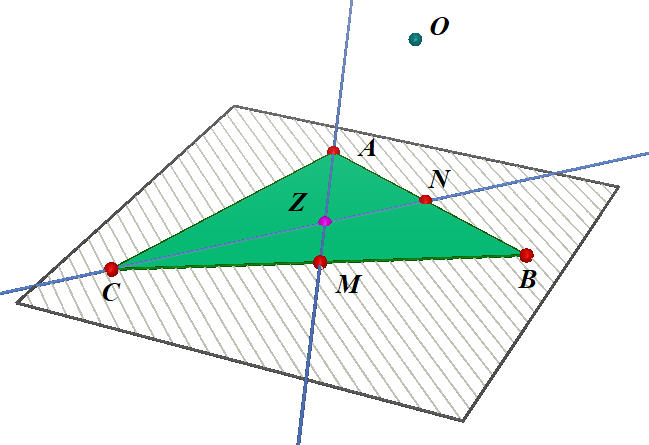
\includegraphics[width=\linewidth]{img/zwaartepunt2.jpg}
\captionof{figure}{Het zwaartepunt van een driehoek}
\label{zwaartepunt2}
\end{center}

Stel de punten $M$ en $N$ gelijk aan de middens van de zijden $[BC]$ en $[AB]$. Dan vinden we het snijpunt $Z$ van de zwaartelijnen door $M$ en $N$ door het volgende stelsel op te lossen van twee vectoriële vergelijkingen:

\[ \left\{ 
	\begin{aligned}
	& \vec{P}=(1-k) \vec{A} + k \vec{M} \\
	& \vec{P}=(1-l) \vec{C} + l \vec{N}
	\end{aligned}
\right.. \]
 
 Door gelijkstelling van de rechterleden en door gebruik te maken van de formule voor het zwaartepunt van een lijnstuk vinden we:
 \[(1-k) \vec{A} + k \frac{\vec{B}+\vec{C}}{2}=(1-l) \vec{C} + l \frac{\vec{A}+\vec{B}}{2}.\]

Herschikken en groeperen van de termen via de eigenschappen van de vectorruimte geeft:
\[ \left( 1-k-\frac{l}{2} \right) \vec{A}+\left(\frac{k}{2}-\frac{l}{2}\right) \vec{B}+\left(\frac{k}{2}+l-1 \right) \vec{C}=\vec{O}.\]

Vanaf hier zijn er twee mogelijkheden om verder te gaan. Het punt $O$ heeft immers nog geen plaats toegewezen gekregen. 

Ofwel leg je $O$ ergens willekeurig buiten het vlak van driehoek $ABC$. In dit geval mag je er van uit gaan dat de vectoren $\vec{OA}$, $\vec{OB}$ en $\vec{OC}$ lineair onafhankelijk zijn. Zo niet dan zouden de punten $A$, $B$ en $C$ collineair zijn en dan zouden de punten $A$, $B$ en $C$ geen driehoek vormen.

Wil je de berekening uitschrijven vanuit het standpunt van een platlander, dan rijzen er praktische bezwaren wanneer je het punt $O$ buiten het vlak van de driehoek moet kiezen. Een platlander kent alleen het vlak waarin hij leeft. In dit geval identificeer je $O$ best met een van de hoekpunten van de driehoek. Neem bijvoorbeeld $O=A$. Je kunt dan steunen op de lineaire onafhankelijkheid van de vectoren $\vec{OB}$ en $\vec{OC}$. De twee berekeningen bij beide opties verlopen analoog.

We gaan verder met de eerste optie: de vectoren $\vec{OA}$, $\vec{OB}$ en $\vec{OC}$ zijn lineair onafhankelijk. Door de onafhankelijkheid van de vectoren komen we dan tot het volgende stelsel:

\[ \left\{ 
	\begin{aligned}
	& 1-k-\frac{l}{2} =0 \\
	& \frac{k}{2}-\frac{l}{2}=0 \\
	& \frac{k}{2}+l-1=0
	\end{aligned}
\right. \]

dat slechts één oplossing heeft: $k=\frac{2}{3}$ en $l=\frac{2}{3}$. Vullen we deze waarden in een van de vergelijkingen van het bovenstaande vectorstelsel in dan vinden we de volgende uitdrukking voor het zwaartepunt van de gegeven driehoek:
\[\vec{Z}=\frac{\vec{A}+\vec{B}+\vec{C}}{3}.\]

Dit is wat we verwacht hadden: een zwaartepuntsformule die analoog is aan de zwaartepuntsformule van een lijnstuk. Maar we kunnen meer besluiten uit deze berekening. De parameterwaarden voor $k$ en $l$ zijn gelijk aan $\frac{2}{3}$ in het zwaartepunt. Dit betekent dat de zwaartelijnen door het zwaartepunt verdeeld worden in lijnstukken die zich verhouden als 2 tot 1. Het deel aan de kant van het hoekpunt is dubbel zo lang als het andere.

Tot slot is er nog een stelling, die we er bij deze berekening gratis bovenop krijgen. Als de zwaartelijnen door $A$ en door $C$ elkaar in een vast punt van deze eerste zwaartelijn snijden, zullen we analoog ook kunnen berekenen dat de zwaartelijnen door $A$ en door $B$ elkaar in ditzelfde vaste punt van de zwaartelijn door $A$ snijden. De drie zwaartelijnen van een driehoek gaan dus door één punt. Dit wisten we allang. Maar het is leuk het nog eens op een andere manier bewezen te zien.


\subsection{Zwaartepunt van een viervlak}
Vooruit nu naar het viervlak $ABCD$ in de driedimensionale ruimte.

\begin{center}
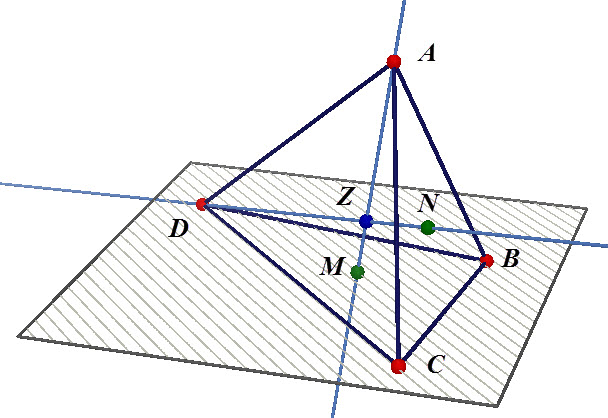
\includegraphics[width=\linewidth]{img/zwaartepunt3.jpg}
\captionof{figure}{Het zwaartepunt van een viervlak}
\label{zwaartepunt3}
\end{center}

Het punt $M$ in figuur \ref{zwaartepunt3} is het zwaartepunt van driehoek $BCD$ en het punt $N$ is het zwaartepunt van driehoek $ABC$. Vectoriële uitdrukkingen voor deze twee zwaartepunten stelden we op in 5.2. Het snijpunt van de zwaartelijnen vinden we nu door de vectoriële vergelijkingen van deze zwaartelijnen in een stelsel onder te brengen:

\[ \left\{ 
	\begin{aligned}
	& \vec{P}=(1-k) \vec{A} + k \vec{M} \\
	& \vec{P}=(1-l) \vec{D} + l \vec{N}
	\end{aligned}
\right.. \]

Na gelijkstelling en substitutie vinden we:
 \[(1-k) \vec{A} + k \frac{\vec{B}+\vec{C}+\vec{D}}{3}=(1-l) \vec{D} + l \frac{\vec{A}+\vec{B}+\vec{C}}{3}\]
 waaruit op de klassieke wijze volgt dat:
 \[ \left( 1-k-\frac{l}{3} \right) \vec{A}+\left(\frac{k}{3}-\frac{l}{3}\right) \vec{B}+\left(\frac{k}{3}-\frac{l}{3}\right) \vec{C}\]
 \[+\left(\frac{k}{3}+l-1 \right) \vec{D}=\vec{O}.\]

Wanneer ik deze berekening op het bord breng, sta ik altijd weer in dubio. Ik kan de oorsprong kiezen binnen de driedimensionale ruimte, bijvoorbeeld door $O$ te identificeren met het punt $C$. De derde term uit de vergelijking valt dan weg en de verdere berekening van het zwaartepunt is precies dezelfde als in de tweedimensionale versie.

Met het oog op de uitbreiding naar hogere dimensies is het echter beter om de oorsprong buiten de driedimensionale ruimte van de tetraëder te kiezen. Niet alle leerlingen zijn echter breeddenkend genoeg om een stapje buiten de bekende driedimensionale wereld te willen zetten. Als er een grote terughoudendheid is ten opzichte van deze onbekende wereld, tracht ik de leerlingen eerst te overtuigen met precedenten, met wiskundige begrippen die alleen maar kunnen aanvaard worden bij de gratie van breeddenkendheid. Ooit hebben de leerlingen allemaal aanvaard dat het getal $\pi$ een echt getal was, niettegenstaande niemand ooit de hele decimale staart had uitgeschreven. Ooit hebben alle leerlingen complexe getallen aanvaard, niettegenstaande er niet eens plaats was voor deze getallen op de getallenas...

Eens de vrees voor de vierde dimensie weggenomen is, leg ik uit dat de keuze van de oorsprong $O$ buiten de drie dimensies van de tetraëder $ABCD$ ervoor zorgt dat de vectoren $\vec{OA}$, $\vec{OB}$, $\vec{OC}$ en $\vec{OD}$ lineair onafhankelijk zijn. In een vierdimensionale ruimte kan dit. Vier vectoren die volledig onafhankelijk van elkaar gekozen zijn, zijn lineair onafhankelijk in de vierdimensionale ruimte. In de driedimensionale ruimte was het maximale aantal lineair onafhankelijke vectoren gelijk aan drie. 

Door gebruik te maken van de lineaire onafhankelijkheid van de vectoren komen we tot het volgende stelsel

\[ \left\{ 
	\begin{aligned}
	& 1-k-\frac{l}{3} =0 \\
	& \frac{k}{3}-\frac{l}{3}=0 \\
	& \frac{k}{3}-\frac{l}{3}=0 \\
	& \frac{k}{3}+l-1=0
	\end{aligned}  
	\right. \]
	
met als enige oplossing $k=\frac{3}{4}$	en  $l=\frac{3}{4}$. Hieruit volgt op dezelfde manier als hierboven dat

\[\vec{Z}=\frac{\vec{A}+\vec{B}+\vec{C}+\vec{D}}{4},\]

dat de vier zwaartelijnen uit de hoekpunten van de tetraëder concurrent zijn en dat ze elkaar doorsnijden in twee lijnstukken die zich verhouden als 1 tot 3. Het gedeelte dat het dichtst bij een hoekpunt van de tetraëder gelegen is, is drie keer zo lang als het andere.

\subsection{Zwaartepunt van een 4-simplex}

Met de voorgaande redenering en berekening eindigt de les over zwaartepunten. De deuren naar de vierde dimensie zijn nu opengezet. Als er leerlingen zijn die het willen proberen, kunnen die het zwaartepunt berekenen van de 4-simplex $ABCDE$. Ze kunnen de berekening sec uitvoeren, zonder toevoeging van een tekening. Een tekening zou hier geen steun meer bieden. 

Er zitten geen onverwachte wendingen in deze berekening. De vectoriële vergelijkingen van twee zwaartelijnen worden opgesteld. Het snijpunt van de zwaartelijnen wordt gevonden door gelijkstelling van de rechterleden. Zo komen ze tot de betrekking:

\[ \left( 1-k-\frac{l}{4} \right) \vec{A}+\left(\frac{k}{4}-\frac{l}{4}\right) \vec{B}+\left(\frac{k}{4}-\frac{l}{4}\right) \vec{C}\]
 \[+\left(\frac{k}{4}-\frac{l}{4}\right) \vec{D}+\left(\frac{k}{4}+l-1 \right) \vec{E}=\vec{O}.\]
 
Door te steunen op de lineaire onafhankelijkheid van de vijf vectoren in de vijfdimensionale ruimte vinden ze de voorspelbare waarden van $k$ en $l$, namelijk $\frac{4}{5}$, en vinden ze de uitdrukking voor het zwaartepunt:

\[\vec{Z}=\frac{\vec{A}+\vec{B}+\vec{C}+\vec{D}+\vec{E}}{5}.\]

\subsection{Doortrekken van formules}

Doortrekken van formules naar hogere dimensies kan soms eenvoudig zijn. Denken we maar aan de formule voor de afstand tussen twee punten of de formule voor het zwaartepunt van een simplex. Maar meestal is er behoorlijk geavanceerde wiskunde nodig om analoge formules te ontwikkelen in hogerdimensionale ruimten. Hieronder geef ik enkele voorbeelden.

De inhoud van een regelmatige $n$-simplex waarvan alle ribben gelijk zijn aan de lengte-eenheid kan berekend worden via determinanten. Het resultaat is:
\[I(n)=\frac{\sqrt{n+1}}{n! \cdot \sqrt{2^n}}.\]

Via meervoudige integralen in poolcoördinaten en via de gamma-functie kan de inhoud bepaald worden van de eenheidsbol in de $n$-dimensionale ruimte:
\[I(n)=\frac{\pi^{\frac{n}{2}}}{\Gamma(\frac{n}{2}+1)}\]
waarbij
\[\Gamma(x)= \int\limits_{0}^{\infty} t^{x-1} e^{-t} \textrm{d}t.\]
Deze behoorlijk ingewikkelde formules laten zien hoe (on)toegankelijk de hogerdimensionale meetkunde is voor de hedendaagse wiskundige. En ze laten de leerlingen met wiskundige aspiraties ook een beetje wegdromen ...

\newpage

\section{Flatland}
Wanneer je het in de klas hebt over hogere dimensies, dan is het een aanrader om kort het prachtige boek \emph{Flatland: A Romance of Many Dimensions} te bespreken. Deze satire werd in 1884 geschreven door de Engelse leraar Edwin Abbott Abbott. 

\begin{center}
	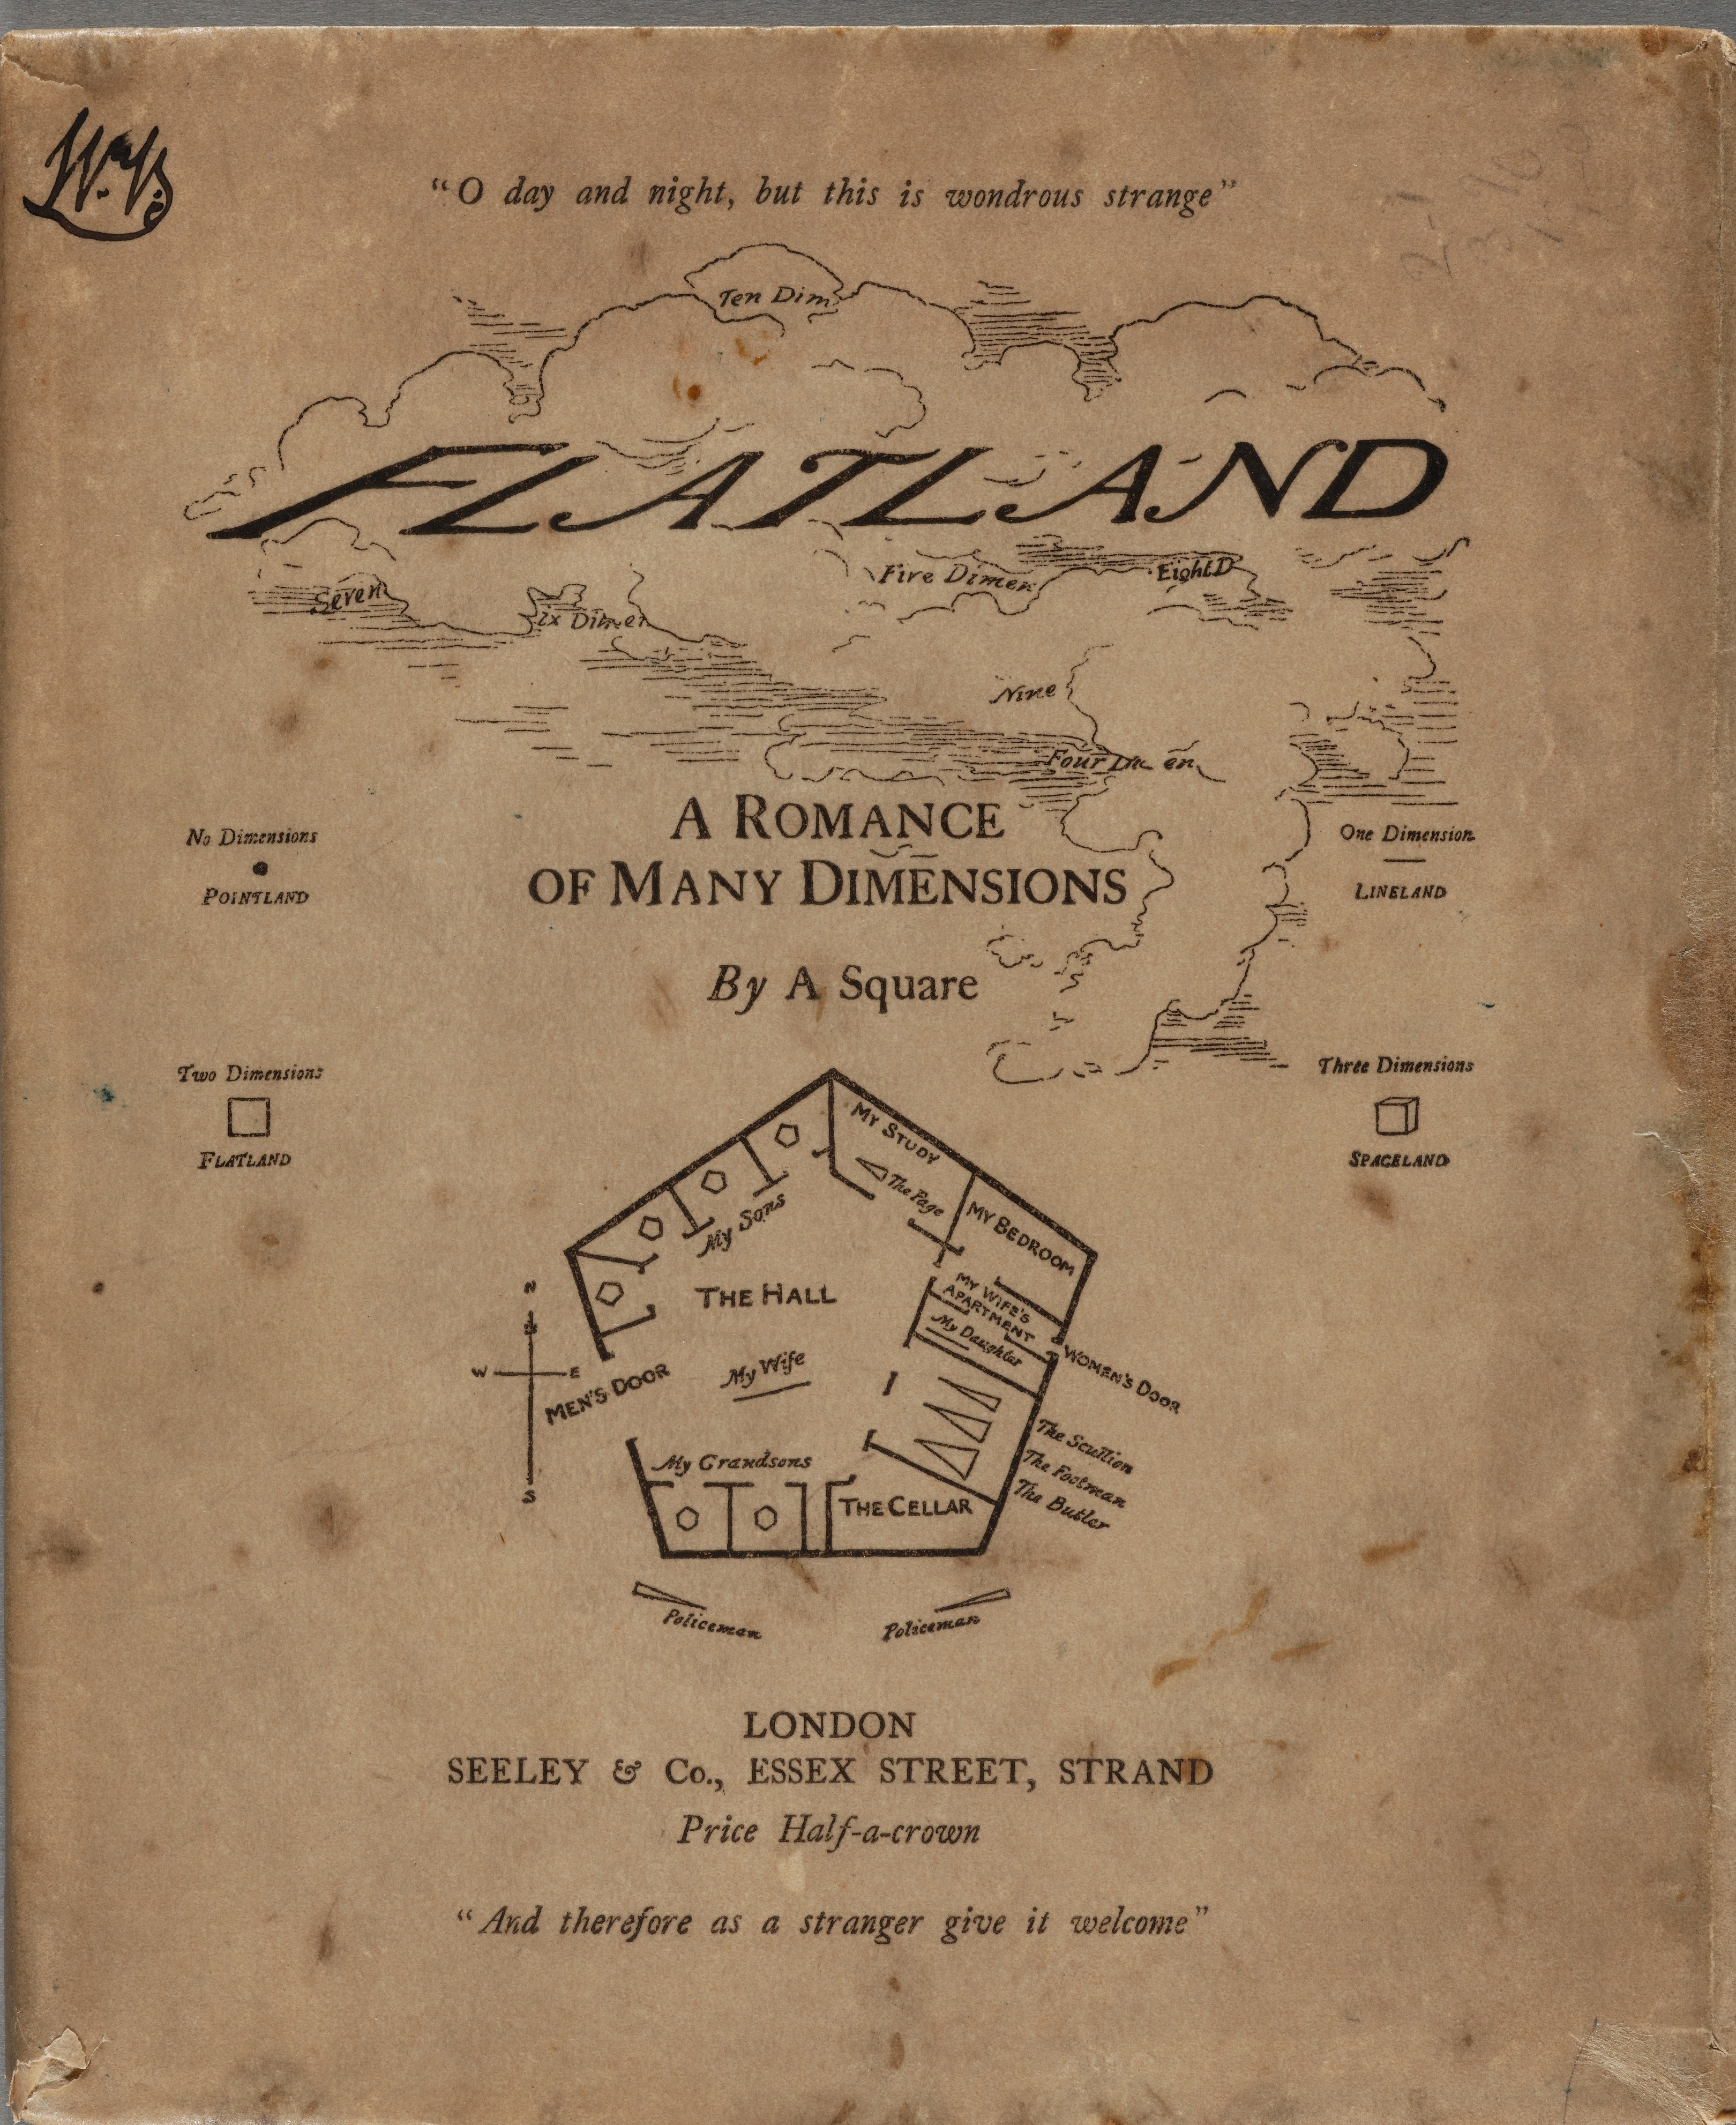
\includegraphics[width=\linewidth]{img/Flatland_cover.jpg}
	\captionof{figure}{De cover van de eerste editie van Flatland (bron: EC85 Ab264 884f, Houghton Library, Harvard University)}
	% noot voor Hilde en Michel: deze foto komt van Wikipedia en bij de uitleg over de rechten op deze foto staat dat er op bovenstaande manier moet naar verwezen worden.
	\label{flatland}
\end{center}

Het boekje wordt nog steeds uitgegeven, maar je kunt het gemakkelijk online vinden. Dat geldt ook voor de Nederlandse vertaling, Platland: een Roman van Vele Dimensies, die al in 1886 verscheen.

In Flatland is het hoofdpersonage en tegelijk de verteller een tweedimensionaal wezen, A Square (Een Vierkant in de Nederlandse vertaling). In het eerste deel van het boek wordt de tweedimensionale wereld van A Square uitgebreid beschreven. De bewoners zijn vlakke figuren die variëren van cirkels, over veelhoeken tot eenvoudige lijnstukken. Hun huizen worden beschreven, hun leefgewoonten... zelfs gedragsregels. De geometrische vormen van de bewoners hangen samen met een soort van kastensysteem. Leerlingen smullen ervan wanneer je dit beschrijft in de klas. Alle platlanders zijn veelhoeken en hun sociale status wordt bepaald door hun aantal hoeken en hun regelmatigheid, met de Cirkel als de perfecte vorm. Soldaten en werklieden van de laagste soort zijn gelijkbenige driehoeken met een heel kleine basis en een scherpe top. Dat is gevaarlijk want een platlander die zo'n gelijkbenige driehoek naar zich ziet toekomen, kan die top moeilijk herkennen en kan er zich aan verwonden als hij niet oplet. Probeer je maar eens voor te stellen hoe je een gelijkbenige driehoek kunt waarnemen in een platte wereld!  De middenklasse van Flatland bestaat uit gelijkzijdige driehoeken. Dokters, advocaten, ambtenaren... zijn vierkanten of regelmatige vijfhoeken. Daarboven staat de adel, onderverdeeld in verschillende graden vanaf de lagere adel, de zeshoeken. Naarmate je naar de hogere adel gaat, neemt het aantal hoeken toe tot je uiteindelijk de eretitel van polygoon kunt krijgen. Als het aantal zijden zo groot wordt en de zijden zo klein dat een veelhoek niet van een cirkel te onderscheiden is, wordt hij ingelijfd in... Ik laat mijn leerlingen hier altijd raden: welke zou de allerhoogste stand kunnen zijn in de 19de eeuwse maatschappij? Sommigen kunnen het raden: de priesterstand!

De bewoners van platland kunnen evolueren volgens een soort van natuurwetten. Zo bijvoorbeeld heeft een zoon één zijde meer dan zijn vader zodat elke generatie klimt op de standenladder. Deze regel geldt echter niet voor de laagste standen van de krijgslieden en de ambachtslui (die, hoe verschrikkelijk, zelfs onregelmatig zijn). Zij kunnen niet opklimmen, tenzij zij heel uitzonderlijke prestaties verrichten, zoals schitterende militaire zeges behalen. Dan kan hun basis misschien iets vergroten zodat zij iets meer regelmatig worden. En zo zijn er nog heel wat sociale regels die uitgebreid beschreven worden door Abbott. Ze zijn een metafoor voor de sociale verhoudingen in de Victoriaanse maatschappij van zijn tijd en hij fileert en bekritiseert die genadeloos. Ik beschrijf in mijn lessen de  laagste klasse van platland steeds aan het eind. Welke groep zou van de allerlaagste stand zijn, nog lager dan de heel simpele werklui en soldaten? Vaak hebben leerlingen geen enkel idee. Weet jij het, beste lezer?

\end{multicols}
\begin{center}
	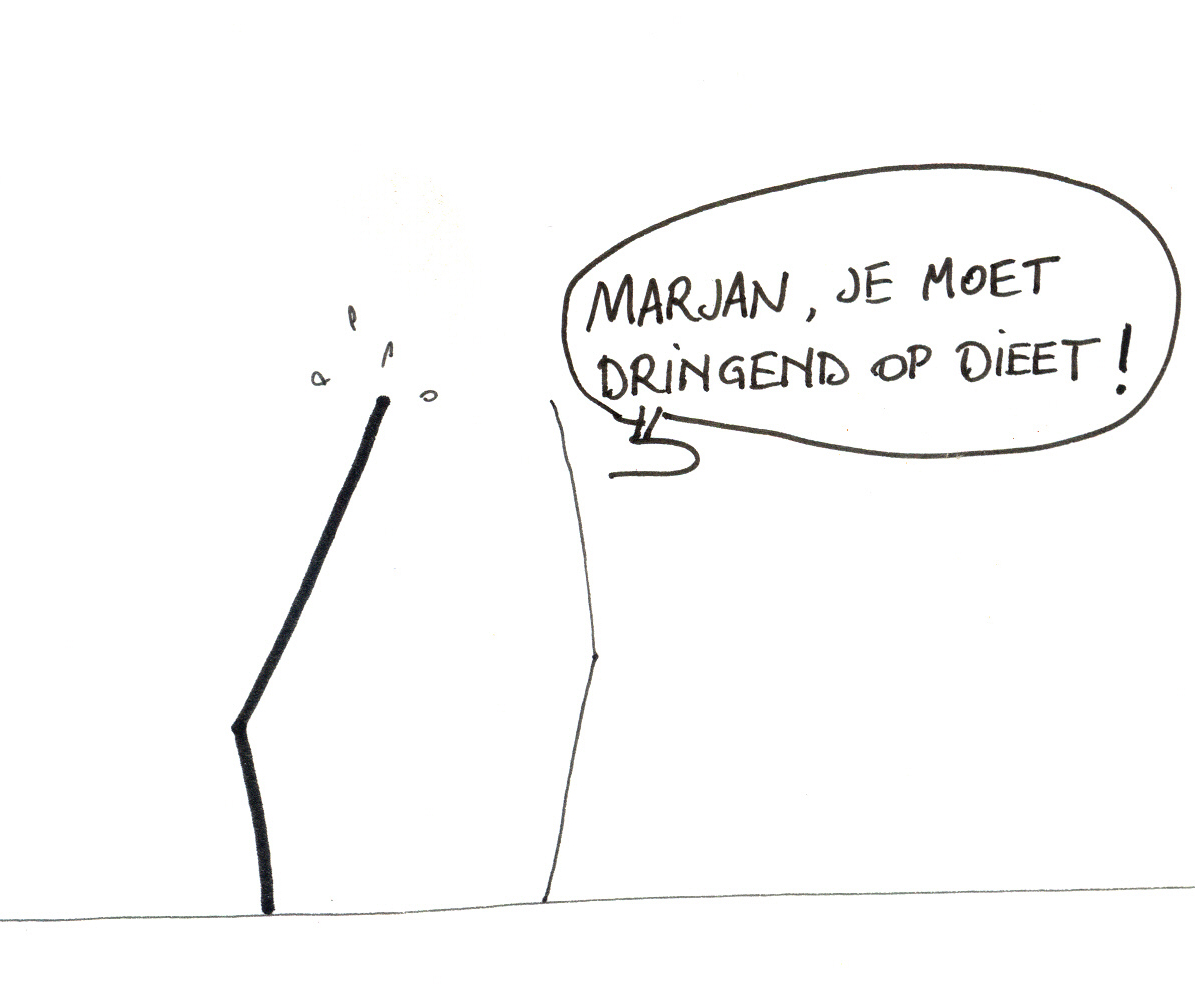
\includegraphics[width=0.65\linewidth]{img/UW mei flatland2.jpg}
	\end{center}
\begin{multicols}{2}

Het zijn de vrouwen! Zij hebben een tophoek die zó scherp is en een basis die zó klein is dat ze niet langer een driehoek vormen, maar een lijnstuk. Als je dat in platland recht op je ziet afkomen, zie je niets (een punt, maar dat is zo klein dat je het niet ziet). Dat lijnstuk is zo scherp dat je je er erg kunt aan verwonden; het kan zelfs dodelijk zijn. Vrouwen zijn dus uiterst gevaarlijk en gemeen. Om die reden zijn er in het wetboek speciale gedragsregels voor vrouwen. We citeren hieronder uit de Nederlandse vertaling de hoofdbepalingen uit dat wetboek.
\begin{quote}
	1. Ieder huis zal een ingang in de oostzijde hebben uitsluitend voor de
	vrouwen, waar alle vrouwelijke wezens `op een welvoegelijke, eerbiedige
	wijze' zullen binnen gaan en niet door de westelijke- of mannendeur.\\
	
	2. Geen vrouwelijke persoon mag op een openbare plaats wandelen zonder
	aanhoudend een waarschuwend `opgepast' te doen hooren op straffe des doods.\\
	
	3. Elke vrouwelijke persoon, die deugdelijk gebleken is te lijden aan
	St. Vitusdans, stuipen, chronische verkoudheid gepaard met hevig niezen
	of eenige ziekte, die onwillekeurige bewegingen veroorzaakt, zal oogenblikkelijk omgebracht worden.
\end{quote}
\setlength{\parskip}{1em}

In sommige staten is er zelfs een aanvullingswet die vrouwen verplicht om op openbare plaatsen heel de tijd met hun achterwerk heen en weer te zwiepen zodat de platlanders hen goed zien aankomen. Schitterend toch! Dit geeft de gelegenheid om in de les wiskunde ook een beetje maatschappijkritiek mee te geven.       

Het tweede deel van het boek beschrijft een manier om naar dimensies te kijken. Het sociale aspect komt hier minder aan bod. Nadat de algemene relativiteitstheorie van Albert Einstein in 1916 werd gepubliceerd en het concept van de vierde dimensie populair werd bij de grote massa, werd het boek van Abbott herontdekt, precies omwille van het tweede deel.

Op Nieuwjaarsavond heeft A Square een droom waarin hij een bezoek brengt aan Lijnland dat bewoond wordt door vreemde punten. Zij kunnen A Square alleen maar zien als een verzameling punten op een lijn en A Square probeert hen er van te overtuigen dat er een tweede dimensie is. Tevergeefs: de koning van Lijnland vindt de ideeën van A Square gevaarlijke nonsens en probeert A Square daarom te vermoorden. Ook Lijnland is heel origineel en soms erg grappig beschreven en geïllustreerd in het boek. Het lezen van die beschrijving, verplicht om grondig na te denken over dimensies.

\end{multicols}

\begin{center}
	\includegraphics[width=0.8\linewidth]{img/lijnland.png}
	\captionof{figure}{Beschrijving van Lijnland in de Nederlandstalige uitgave van Flatland}
    \label{lijnland}
\end{center}

\begin{center}
	\includegraphics[width=0.8\linewidth]{img/bol_door_platland.png}
	\captionof{figure}{Een bol reist door Platland }
	\label{bol}
\end{center}
\setlength{\parskip}{1em}

\begin{multicols}{2}

Een tijdje na het visioen van Lijnland, wordt A Square bezocht door een driedimensionale bol. Natuurlijk ziet het arme vierkant deze bol slechts als een cirkel die groter en kleiner wordt naarmate de bol door Platland beweegt. Hiervan is een mooie tekening opgenomen in het boek, zie figuur \ref{bol}. A Square kan moeilijk geloven dat er zoiets bestaat als drie dimensies en is maar echt overtuigd wanneer hij door de bol wordt meegenomen naar de driedimensionale ruimte en Spaceland (Ruimteland) met zijn ogen ziet.





 Elk jaar bezoekt de bol het vierkant in de hoop van die laatste een soort apostel te maken die de platlanders kan onderwijzen en overtuigen van het bestaan van een derde dimensie. Maar A Square denkt zelfs verder door: als de lijnlanders het bestaan van twee dimensies niet kunnen vermoeden en de platlanders hetzelfde probleem hebben met drie dimensies, kan de bol er dan wel zeker van zijn dat er niet een vierde dimensie is of nog hogere dimensies? En is er misschien een Puntland? Duizelingwekkende vragen, ook voor de bol die de gedachte aan vier dimensies resoluut afwijst.

Hoe de ontdekkingsreis van A Square door hogere dimensies verloopt en hoe het uiteindelijk afloopt met A Square, moet je verder lezen in het boek Flatland, dat uiteindelijk niets anders blijkt dan de memoires van het vierkant. Een juweeltje!\\


\end{multicols}
\begin{center}
	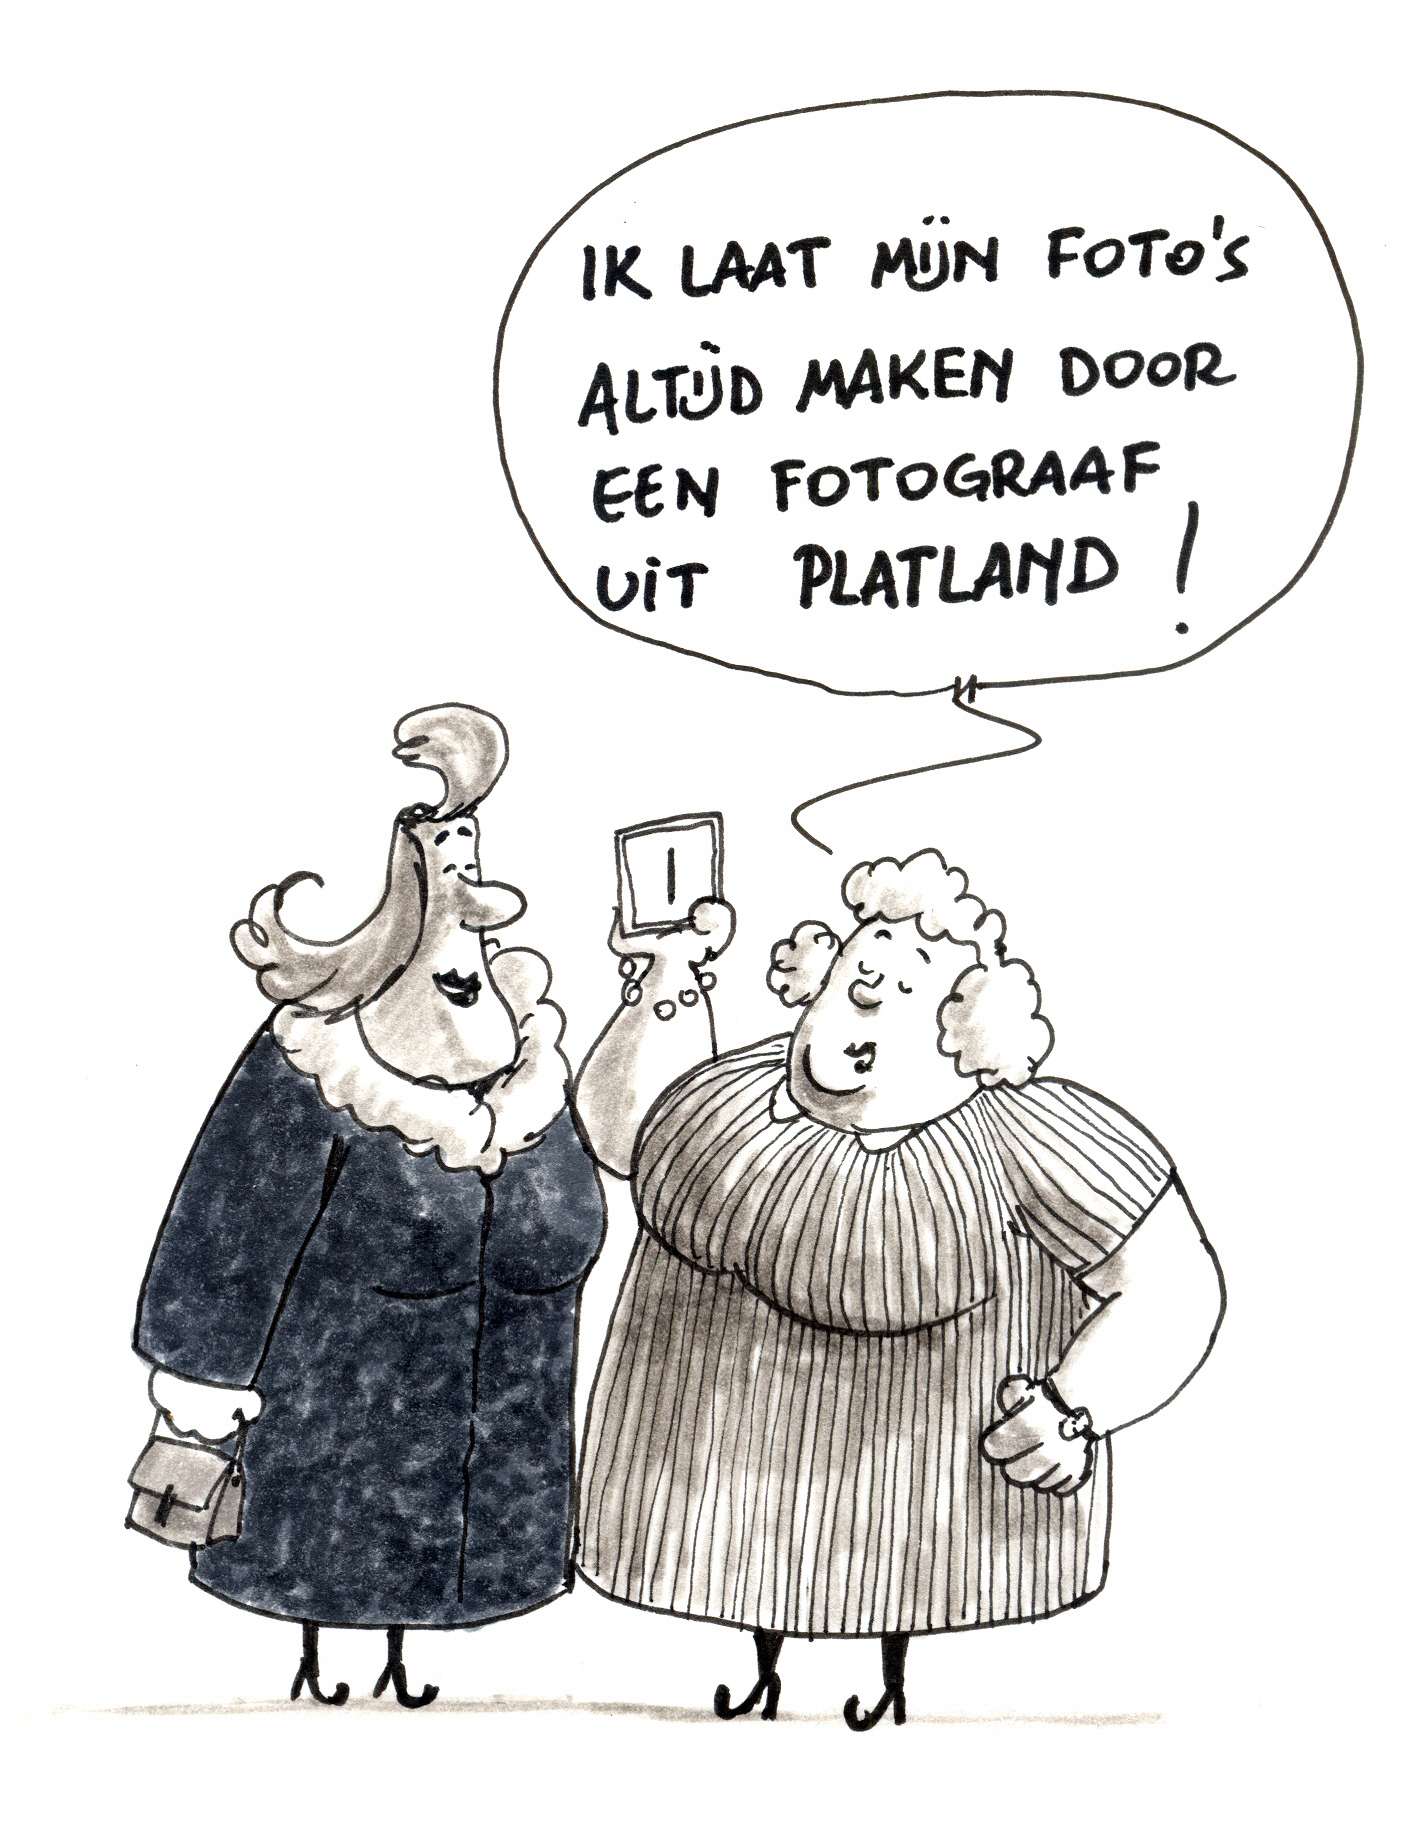
\includegraphics[width=0.65\linewidth]{img/UW mei flatland.jpg}
	\end{center}



\stopcontents[mainsections]			        % altijd laten staan, opsomming in inhoudstafel enkel tot loep beperken


% bronnen toevoegen
\begin{bronnen}
\item Abbott Abbott, E. (1884). \emph{Flatland: A Romance of Many Dimensions}. London:  Seeley \& Co. Heruitgave 1992: Oneworld Publications. ISBN 978-18-5168-086-3.   \url{http://www.geom.uiuc.edu/~banchoff/Flatland/}. Nederlandse vertaling: 
 \emph{Platland: Een Roman van Vele Afmetingen}.   \url{http://www.fisme.science.uu.nl/nwd/nwd2006/handouts/platland.pdf}
 
\item Courant, R. en Robbins, H. (1996). \emph{What is Mathematics?}. Oxford University Press. ISBN 978-0-19-510519-3. 227-234.

\item ElicaTeam. \emph{MathLapse - Monge's Theorem}.\\ \url{https://www.youtube.com/watch?v=CP4AW-b-NiY}

\item Gheysens, L.(2012). \emph{De cirkels van Monge}. \\ \url{http://blogimages.bloggen.be/gnomon/attach/276147.pdf.}.

\item Ib\'a\~{n}ez, R. (2016). \emph{De vierde dimensie, een hogere werkelijkheid van ons universum}. Kerkdriel: Librero b.v. ISBN 978-90-8998-681-8.

\item \emph{Ipuy en zijn vrouw krijgen offergaven van hun kinderen} (ca. 1250 v.C.). [Schilderij]. New York: The Metropolitan Museum of Art. Publiek domein. \url{https://www.metmuseum.org/art/collection/search/548567}

\item Khoury, M. \emph{Counterintuitive Properties of High Dimensional Space}.\\ \url{https://marckhoury.github.io/ counterintuitive-properties-of-high-dimensional-space/}

\item Kindt, M. (1993). Ruimtevisioenen in Platland. \emph{Nieuwe Wiskrant 12/4}, 148-156.

\item Numberphile. \emph{Perfect Shapes in Higher Dimensions}.\\

\item Roelens, M. (1992). De drie cirkels. \emph{Uitwiskeling 8/2}, 4-6.

\item Slepian, Z. (2012). \emph{Average Projected Area of a Convex Solid - Generalization to Higher Dimensions}. \url{https://arxiv.org/pdf/1109.0595.pdf}



\item Tytgat, P. (2010). Meer dan drie dimensies. \emph{Uitwiskeling 26/4}, 9-16.

\item Union College. \emph{Folding a hypercube}.\\ \url{http://www.math.union.edu/~dpvc/math/4D/folding/hcube-folding.html}

\item Van den Broeck, L. \emph{De octaëder in de vierdimensionale ruimte}.\\ \url{https://www.youtube.com/watch?v=6gDCIrJSZ6g}


\item Wikipedia. \emph{Tesseract}. \url{https://en.wikipedia.org/wiki/Tesseract}

 \url{https://www.youtube.com/watch?v=2s4TqVAbfz4}
 


\end{bronnen}


\vspace{7ex}



\begin{kader}
\emph{Hoe werk je op een onderzoekende manier met statistiek in je klas?}
\vspace{2ex}

\emph{Kun je leerlingen van de eerste graad warm maken voor data?}

\vspace{2ex}
\emph{En hoe gebruik je ICT doeltreffend en tijdsefficiënt in de lessen statistiek?}

\vspace{2ex}

De \textbf{nieuwe eindtermen statistiek} voor de eerste graad secundair zijn best ambitieus. Dat hoort zo, want wie statistiek in de vingers heeft, staat sterker in zijn/haar schoenen. Onze datagedreven maatschappij overspoelt ons met informatie en gegevens waar we bewust moeten mee leren omgaan.

\begin{multicols}{2}

Het boek \textbf{‘Straf in statistiek’} wil leerkrachten inspireren om op een natuurlijke, onderzoekende manier met statistiek aan de slag te gaan. Leerlingen zinvol aan het werk zetten is daarbij de rode draad. Het boek maakt de link met de dagelijkse realiteit en toont hoe je Google Forms en Excel inzet om data te verzamelen en te verwerken. Met de gedetailleerde, stapsgewijze handleidingen, datasets en online screencasts ga je meteen aan de slag en neem je vol enthousiasme je leerlingen mee op sleeptouw.
\vspace{2ex}

‘Straf in statistiek: Laat je leerlingen werken met data en digitale tools’: vanaf nu verkrijgbaar bij Acco: \url{www.acco.be/statistiek}
\begin{center}

\includegraphics[width=0.55\linewidth]{img/boek statistiek.JPG}
\end{center}
\end{multicols}
\end{kader}